\documentclass[12pt,a4paper]{report}
\usepackage[paper=a4paper]{geometry}% http://ctan.org/pkg/geometry
\usepackage[english]{babel}
\usepackage[T1]{fontenc}

\usepackage{makecell}
\usepackage{pdfpages}
\usepackage{tikz}
\usetikzlibrary{calc}
\usepackage{fancyvrb}
\usepackage{multicol}
\usepackage{lipsum}
\usepackage{setspace}
\usepackage{soul}
\usepackage{fontspec}
\usepackage{colortbl}
%\usepackage{background}
\usepackage{caption}
\usepackage{pgfgantt}
\usepackage{graphicx}
\usepackage[yyyymmdd]{datetime}

\usepackage{indentfirst} 
\usepackage{pgfgantt}
\usepackage{rotating}
\usepackage[graphicx]{realboxes}
\usepackage[subfigure]{tocloft}
\usepackage{xcolor}
\usepackage{listings}
\usepackage{csquotes}
\usepackage[acronym]{glossaries}


\newdateformat{monthyeardate}{\monthname[\THEMONTH] \THEYEAR}
\newcommand{\listappendicesname}{Appendices}
\newlistof{appendices}{apc}{\listappendicesname}
\newcommand{\appendices}[1]{\addcontentsline{apc}{appendices}{#1}}

\newcommand{\newappendix}[1]{\section*{#1}\appendices{#1}}


\usepackage{titlesec}
\titleformat{\chapter}[display]{\fontsize{24pt}{36pt}\bfseries}{}{5pt}{}
\titleformat{\section}[display]{\fontsize{16pt}{24pt}\bfseries}{}{5pt}{}
\titleformat{\subsection}[display]{\fontsize{14pt}{21pt}\bfseries}{}{5pt}{}


\usepackage{titletoc}
\usepackage{sectsty}
\usepackage{float}
%\usepackage[table,xcdraw]{xcolor}
\usepackage{tocloft}
\renewcommand{\cftsecleader}{\cftdotfill{\cftdotsep}}
\usepackage{afterpage}

\usepackage{listings}
\usepackage{color}
\usepackage{subfigure}


\newcommand\blankpage{%
    \null
    \thispagestyle{empty}%
    \addtocounter{page}{-1}%
    \newpage}
\renewcommand{\baselinestretch}{1.5} 

\addto\captionsenglish{%
  \renewcommand\contentsname{Table of Contents}%
}

\usetikzlibrary{calc}
\newcommand\HRule{\rule{\textwidth}{1pt}}


\newgeometry{top=25mm,bottom=25mm,left=25mm,right=37mm}
\usepackage[nottoc,numbib]{tocbibind}
\usepackage[citestyle=ieee]{biblatex}
\addbibresource{report.bib}

\setlength{\footskip}{20pt}

\setmainfont{Times New Roman}
\makeglossaries
\begin{document}

\begin{titlepage}


\center % Center everything on the page
{

\vspace*{\fill}
\setstretch{1.2}
\fontsize{20pt}{30}\selectfont \textbf{\uppercase{ELECTRINIC KIDNEY RECIPIENTS' REGISTRY}}\\[1.5cm]
\vspace*{\fill}

\fontsize{16pt}{24}\selectfont{B GNANAKEETHAN} \\


\vspace*{\fill}

\fontsize{16pt}{24}\selectfont\textbf{\monthyeardate\today}
}

\vspace*{\fill}

\end{titlepage}

\begin{titlepage}


\center % Center everything on the page
{\setstretch{1.2}

\includegraphics[width=1.5in,height=1.5in,keepaspectratio]{logo.png}\\[0.5cm]
\fontsize{20pt}{30}\selectfont \textbf{\uppercase{ELECTRINIC KIDNEY RECIPIENTS' REGISTRY}}\\[1.5cm]
\fontsize{16pt}{24}\selectfont{B GNANAKEETHAN} \\
\fontsize{16pt}{24}\selectfont{R1812154} \\
\fontsize{16pt}{24}\selectfont{18121548} \\[1cm]

\fontsize{16pt}{24}\selectfont{Name of the Supervisor:} \\[0.5cm]
\fontsize{16pt}{24}\selectfont{Ms. B. Yaalini} \\[0.5cm]


\vspace*{\fill}

\fontsize{16pt}{24}\selectfont\textbf{\monthyeardate\today} \\[0.5cm]


\vspace*{\fill}


\begin{figure}[!h]
  \centering
  \begin{minipage}[b]{0.2\textwidth}
    
\includegraphics[width=1.5in,height=1.5in,keepaspectratio]{bit-logo.png}
  \end{minipage}
  \hfill
  \begin{minipage}[b]{0.2\textwidth}
    
\includegraphics[width=1.5in,height=1.5in,keepaspectratio]{ucsc-logo.jpg}
  \end{minipage}
\end{figure}

\fontsize{12pt}{12}\selectfont \textbf {This dissertation is submitted in partial fulfilment of the requirement of the Degree of Bachelor of Information Technology (external) of the University of Colombo School of Computing}\\[0.5cm]
}

\vspace*{\fill}

\end{titlepage}
\newgeometry{top=20mm,bottom=20mm,left=37mm,right=20mm}


\pagenumbering{roman}

%\section*{Declaration}
\addcontentsline{toc}{chapter}{Declaration}  
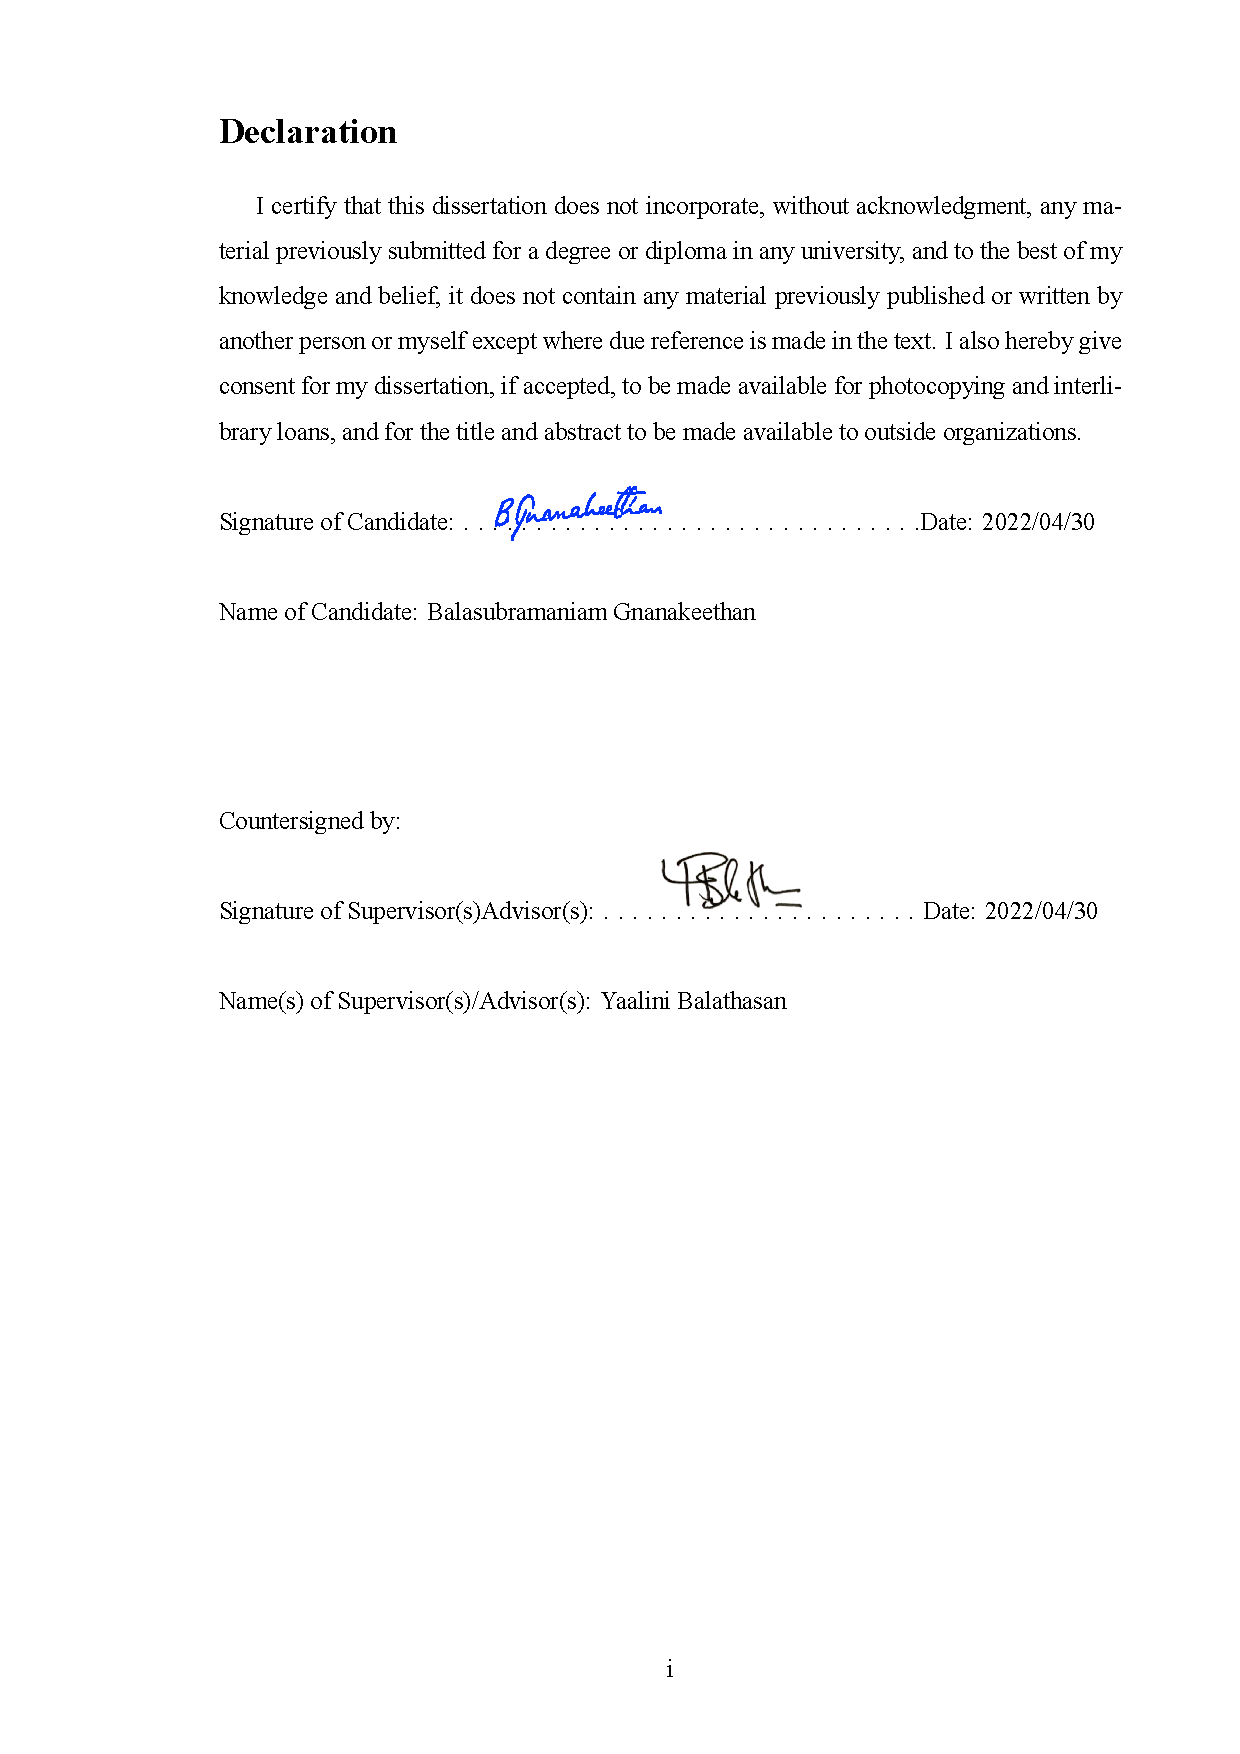
\includepdf{declaration.pdf}
%
%I certify that this dissertation does not incorporate, without acknowledgment, any material previously submitted for a degree or diploma in any university, and to the best of my knowledge and belief, it does not contain any material previously published or written by another person or myself except where due reference is made in the text. I also hereby give consent for my dissertation, if accepted, to be made available for photocopying and interlibrary loans, and for the title and abstract to be made available to outside organizations.\\
%
%\noindent Signature of Candidate: . . . . . . . . . . . . . . . . . . . . . . . . . . . . . . . .Date: \today \\
%
%\noindent Name of Candidate: Balasubramaniam Gnanakeethan\\
%
%\vspace{2cm}
%
%\noindent Countersigned by:\\
%
%\noindent Signature of Supervisor(s)Advisor(s): . . . . . . . . . . . . . . . . . . . . . . Date: \today \\
%
%\noindent Name(s) of Supervisor(s)/Advisor(s): Yaalini Balathasan
%\newpage

\section*{Abstract}
\addcontentsline{toc}{chapter}{Abstract}

Need for a digital health solution in managing end-stage renal disease patients who are awaiting kidney transplants, especially during workup for surgery and in finding a kidney donor was emerging during the last decade in the medical professorial unit in the national hospital of Sri Lanka. It extends toward the patients who got kidney transplants and on clinic follow-up. Lack of online data of kidney recipients when a cadaveric kidney is available, lack of interoperability and good coordination in information exchange between health institutions, difficulties of record-keeping and timely updating, etc were the main emerging difficulties for the health staff to manage. Design and development of an electronic renal registry were initiated along with the need from the stakeholders to provide a better solution for all mentioned difficulties.

The system is being developed using the Iterative Spiral Model of Software Development as the system requirements may change as the system is evolved and presented to the client. It uses Golang as the backend language and PostgreSQL as the database layer. It has a web-based frontend compiled using Svelte Library. The frontend and the backend are interfaced using a GraphQL Specification. 

\newpage

\section*{Acknowledgments}
\addcontentsline{toc}{chapter}{Acknowledgments}

I would like to thank my supervisor Ms. Yaalini Balathasan for her continuous guidance and support throughout the development of the project. I am forever grateful for the appreciation and support from Dr. Roshan Hewapathirana. I also would like to thank Dr. Chamila Malsiri for providing me with valuable information for the implementation of the system. It was a great opportunity to work with all of them. Thank you. 

\newpage


\newpage 
\renewcommand{\baselinestretch}{1.5}\normalsize
\tableofcontents
\addcontentsline{toc}{chapter}{Table of Contents}
%\renewcommand{\baselinestretch}{1.5}\normalsize

\listoffigures
 
\listoftables


\newpage

\pagenumbering{arabic}
%\pagenumbering{gobble}
\setcounter{page}{1}
%\addcontentsline{toc}{section}{Unnumbered Section}


\chapter{Introduction}
\section{Introduction}
%\newacronym{gcd}{GCD}{Greatest Common Divisor}
%
%\newacronym{lcm}{LCM}{Least Common Multiple}
%
%Given a set of numbers, there are elementary methods to compute 
%its \acrlong{gcd}, which is abbreviated \acrshort{gcd}. This 
%process is similar to that used for the \acrfull{lcm}.

The necessity of Digital Health Solutions is emerging in the world due to technological shifts and digital transitions. The need for a digital health solution in the Nephrology Unit of the National Hospital of Sri Lanka was identified in the Postgraduate Institute of Medicine, University of Colombo. The workups for the End-stage renal disease patients and finding a donor for them is a complicated process. The patients who have received kidney transplant needs to have regular follow-ups and investigations to be managed. 

\section{Motivation for the project}
The hospital system faces numerous troubles in the current environment due to the drawbacks of finding recipients when a cadaveric kidney donor is found.  There is less interoperability and good coordination between health institutions that constitute a critical blocker. The main reason is the manual process that involves managing the records and these records are not searchable in the quickest possible manner. Designing and developing an electronic system that can provide these functionalities for the Medical Officers and Doctors is essential.  


\section{Objectives of the project}

\begin{itemize}
\item The system should allow a medical officer to manage a patient 
\item The system should allow a consultant to derive conclusions from the analytical reports of the patient
\item The system should allow a medical officer to find a recipient for a cadaveric donor. 
\item The system should provide analytical information about a patient’s progress in the system. 
	
\end{itemize}


\section{Scope}
The scope of the project is to provide a kidney patients’ registry that allows Consultants and Medical Officers to manage End-Stage Renal Disease patients efficiently. The system will ease manual the process of continuity of care. 

\section{Functional Requirements of the System}

\begin{itemize}
\item The system should allow the recording of the diagnosis history of patients. 
\item The system should assist the Consultants and Medical Officers in taking critical decisions about patients’ health. 
\item The system should alert patients on their potential days of clinic meetings.
\item The system should alert Medical Officers of potential missing patients from a specific clinic day.

\end{itemize}

\section{Non-Functional Requirements of the System}
\begin{itemize}

\item The system should store information in a secure manner not exposed to malicious actors.
\item The system should prevent record tampering. 
\item The system should be available and reliable throughout the process. 
	
\end{itemize}

\newpage
\chapter{Requirement Gathering \& Analysis}

System analysis is an essential phase of a software development project. The process allows us to understand the complexity of the system in concern by sections. Hence it allows for a better understanding of it.  The currently available mechanisms are considered, and their pitfalls and advantages are measured. This provides a better way to achieve the project goals.

\section{Existing Systems}
\subsection{Current Manual Process}

Currently, the Medical Officers and Consultants process the patients through manual processes. There are multiple forms via which data is collected and stored about the patients. 
Patients are issued clinic books in which the patients’ diagnosis records are recorded. The patients usually must carry them with them alongside the other laboratory reports. However, there are significant issues alongside the manual process and it is highly time-consuming for the doctors and the patients. A Serial number is issued for every patient and it is recorded into the registry in the clinic room. The registrar keeps track of the demographic information about the patients. The serial number can be used to trace previous appointments, but however, only clinic books have the medical history of the patient. If the patient loses the clinic book, there are no other means to trace the history of the patient. 

\subsection{Afflo.io}
An off-the-shelf solution called Afflo.io is provided as an on-premise solution for Transplant Management requirements. It has features like Donor management, Patient management comprising of facilities for self-management by patients, Electronic Health Records integrations, and Organ matching features. The system is a fully proprietary system. There is no comparable information from the informational site.  \cite{afflo}


\subsection{OpenTransplant}
The solution is an open-source solution developed in a foreign country with Governmental Assistance. The project has received some recognition from the online community. However, the project primarily focuses on Cadaveric Transplants whereas our system has to focus on Live Donor transplants as well. Besides that our system strives to achieve a feature parity of a similar nature.\cite{opentransplant}

\subsection{Otter Organ(CareDX)}

This is also a commercially available solution. The solution has a full stack of solutions needed to manage organ transplants. This also has necessary features like Organ transplant tracking, research \& reporting features like others. In addition to that, it has a data visualization feature. \cite{otter}



\section{Fact Finding Techniques}

The client’s requirements must be gathered properly to produce an efficient output. Hence there are multiple methods we can use to develop the system. The fact-finding techniques can be critical in the analysis phase of the software development lifecycle. Even though we have multiple methods of fact-finding mechanisms, The relevant information for the development of this system was found via 
\begin{itemize}
	\item Discussions with Open Ended Questions \\
	There were discussions with the Consultants and the medical doctors who are supposed to use the system. Such that they were asked non-specific questions relevant to their needs in a proper digitized solution. Through their answers their requirements were defined.
	\item Semi Structured Interviews \\
	The prospectful users were asked questions on their scope of usage of the system and how they intend to interact in the system, via such methods, their inputs were conceived into a requirements specification. 
\end{itemize}
Through observation of the existing systems and analyzing the consumption patterns, it was determined that the users are relying on them in a specific pattern.  

\section{Feasibility Study for the Proposed System}

The feasibility study is a very important process to find out the strength, weaknesses, threats, and opportunities of the proposed system to fulfill the main requirements. The measure of how beneficial an information system will be to an organization. A feasibility study is used for making accurate decisions. A detailed feasibility study was carried out regarding this system in the following sections.

\subsection{Operational Feasibility}
The operational feasibility of this system is highly important since the system is required to be used by less technical people who would like to achieve their goals very quickly. The operational feasibility measures the context in which the system in question accomplishes the requirement. The hospital is also eager to implement 

\subsection{Technical Feasibility}
The technical feasibility analyses the availability of technical resources and technical expertise to complete the product. The product requires significant technical expertise and effort. 

\subsection{Schedule Feasibility}
The schedule feasibility analyses whether the completion of the product could occur within a defined timeframe providing an advantage to the benefactor of the system. The implementation of the system will highly benefit the hospital in managing its patients effectively. 

\section{Requirements Definition}
The requirement definition is an important part of a software development project. It defines the final requirement that the project/software should address and complete. A clear requirement definition is required for a project to succeed in an effective manner.
\subsection{Functional Requirements}
The functional requirements comprise the very critical requirements which are of absolute necessity for the system to function. A system always has a set of functional requirements. The functional requirements finalized for the system which is being developed are as follows.
\begin{itemize}
\item The Medical Officers should be able to record patient information.
\item The Medical Officers should be able to monitor patient progress.
\item The system should assist the Nephrology Consultants to make proper decisions.
\item The system should be able to provide assistance in matching donors to Medical officers and Nephrology consultants alike.
\end{itemize}






\subsection{Non Functional Requirements}

The non-functional requirements are for non-critical parts of the software. These requirements enhance the experience of the user and provide additional features, however, these features do not affect the core functionality of the system. The following features have been identified as non-functional requirements of the system. 

\begin{itemize}
\item Security – The system must feature security protocols to prevent misuse from malicious users/actors.
\item Usability – The system must be user-friendly. 
\item Reliability – The system must provide a reliable \& consistent interface for medical officers to carry out their duties.
\item Reusability and Maintainability – The system should be able to be reused or maintained / modifiable in the future to fit further requirement changes. 
\end{itemize}

\subsection{Resource Requirements}
This system is designed to be on a central server. Minimum hardware requirements to run the backend system are as follows.
\begin{itemize}
\item Octa-Core 2.5GHz Processor
\item 8GB of RAM
\item 80GB of Storage Space or above. 
\end{itemize}
The system does not have any operating system dependencies. It requires PostgreSQL 14+ Database. It can be consumed by either using a mobile or desktop device via any Internet Browser. 
 
\chapter{Design of the solution}

System design is an important process of defining interfaces, architecture, components, databases, and models necessary for the development of the solution while satisfying system requirements. The system design converts the requirements into a technical solution. The design process is more creative and knowledge-based than system analysis. 

\section{Methodology}

The design of the system can be done using various tooling. The process is very complex, and the designer should have the means to organize a vast amount of information gathered during analysis and determine if there are any discrepancies in the flow of information. 

\begin{figure}[h]
\begin{center}
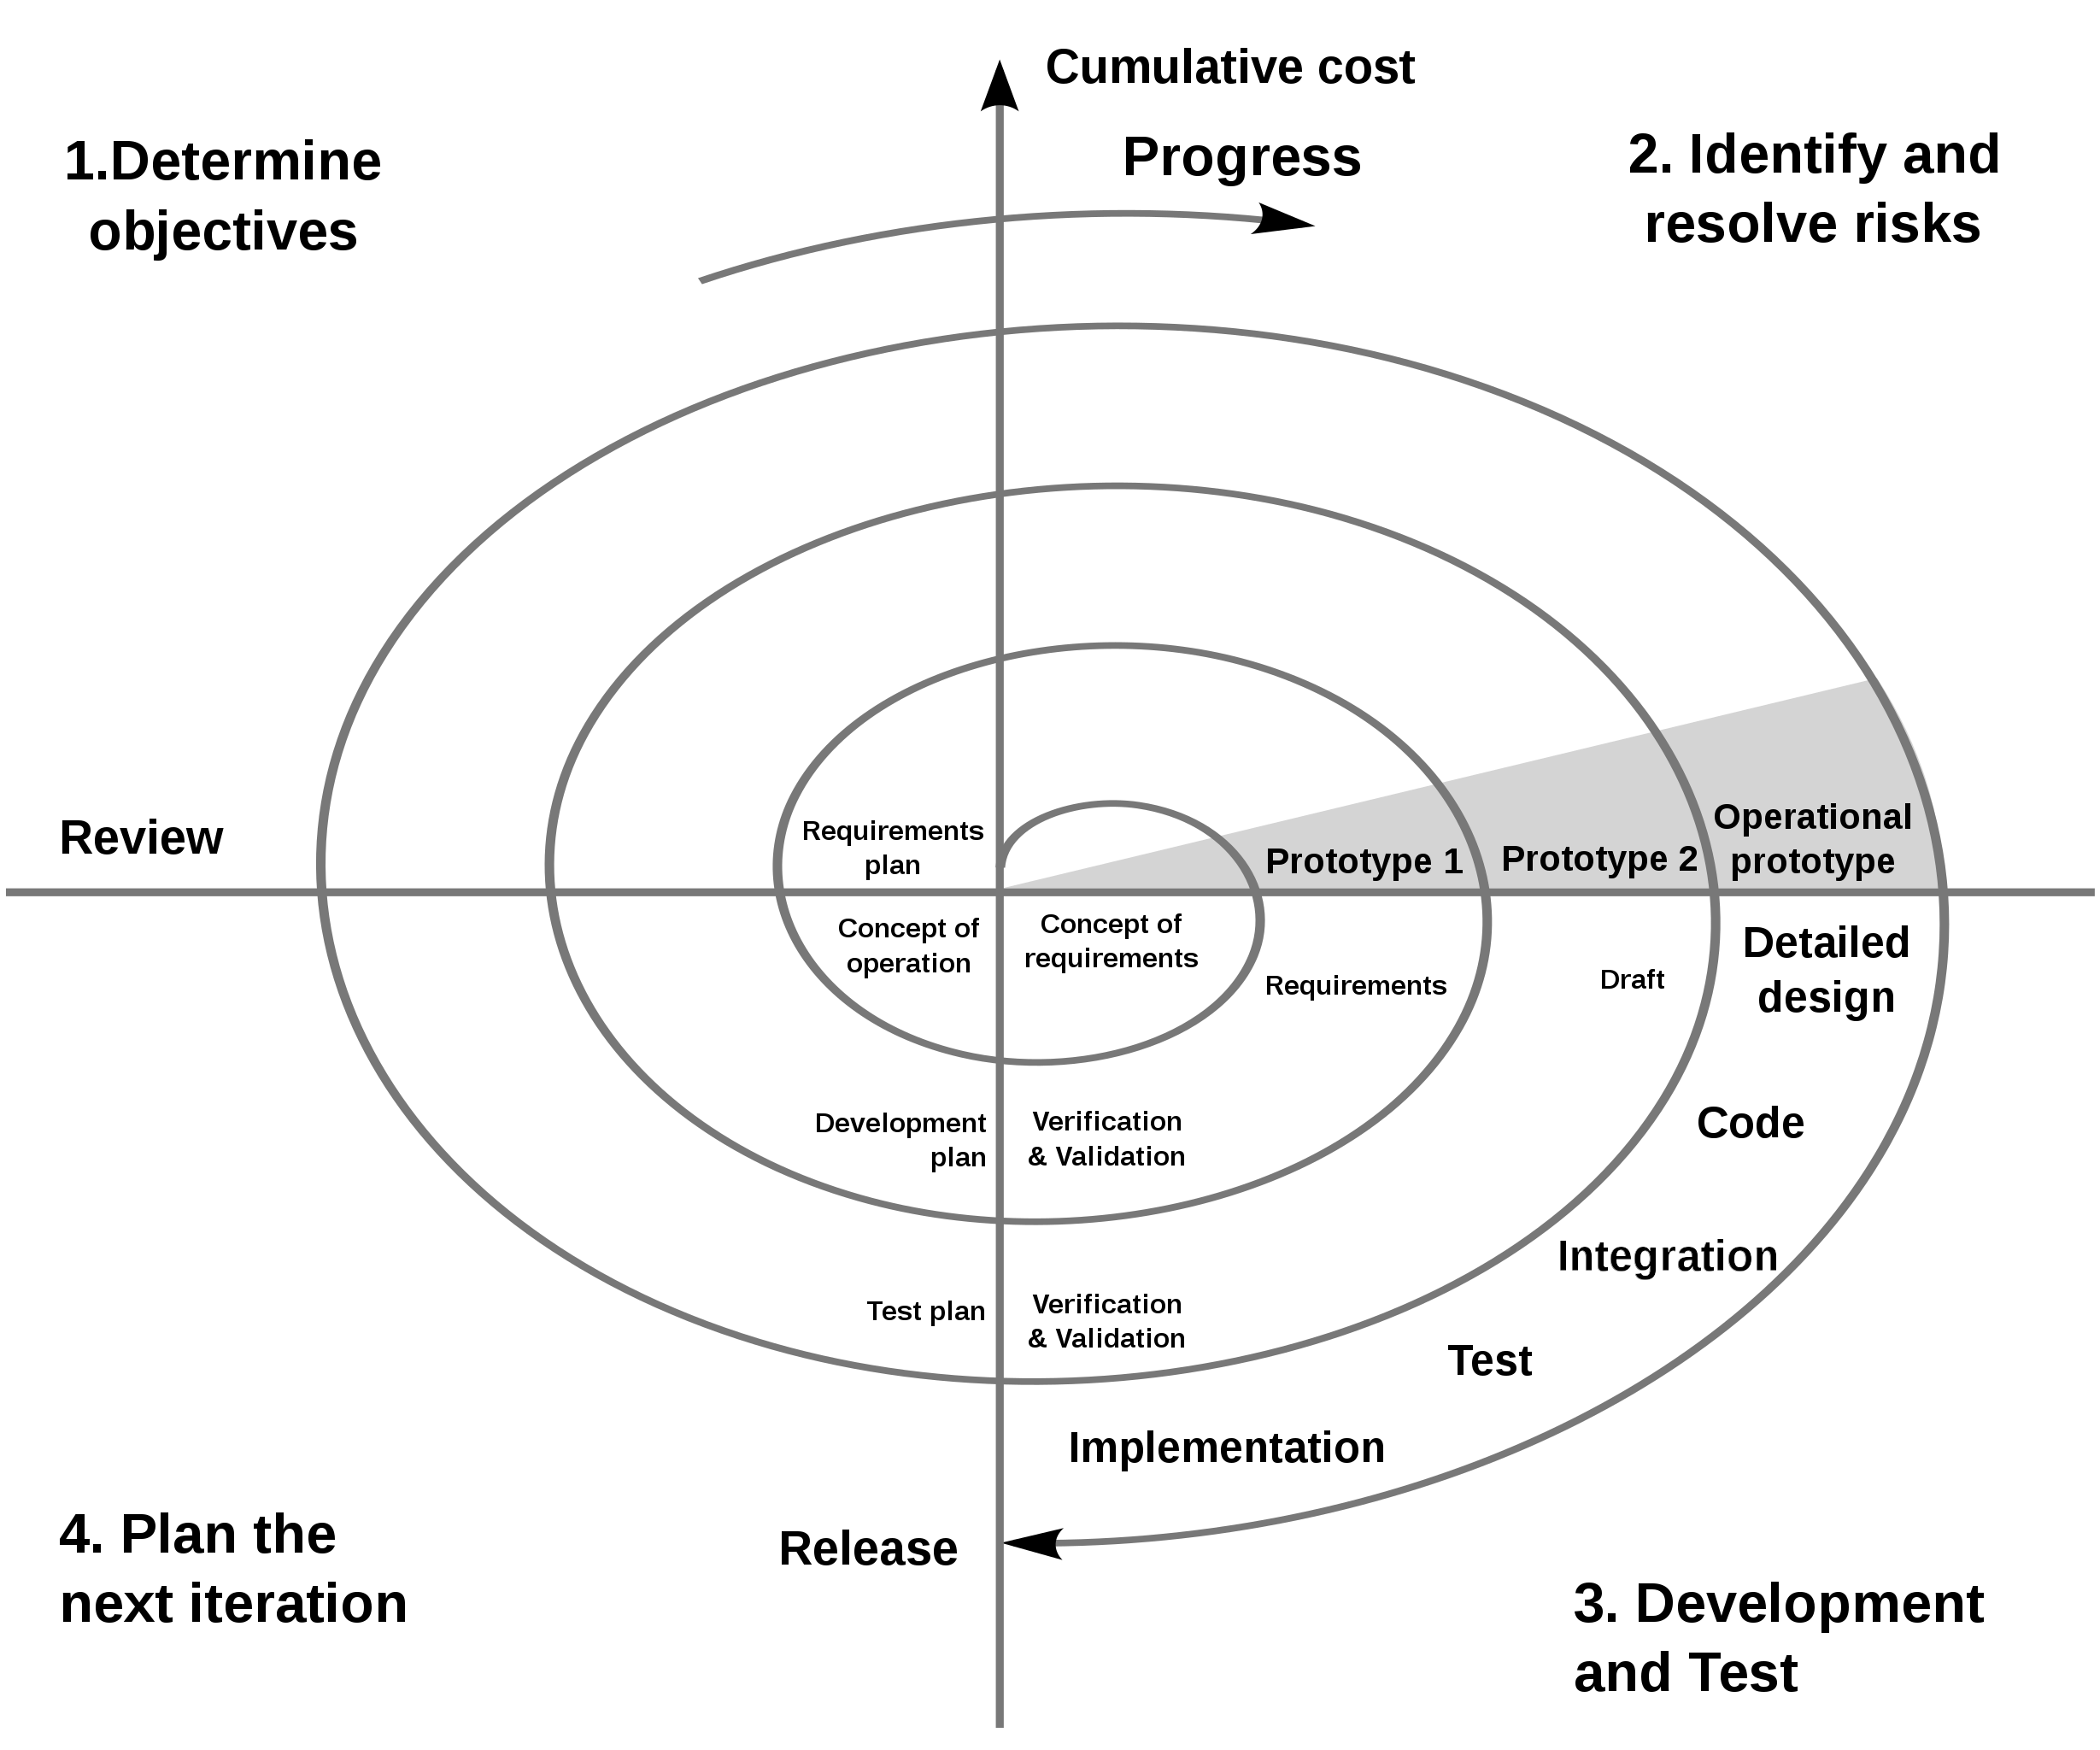
\includegraphics[width=0.8\textwidth]{images/spiral.png}	
\end{center}
\caption{Spiral / Iterative Method}
\label{fig:spiral}
\end{figure}

There are different development methodologies for the software development cycle. Such as the Waterfall method, Spiral /Iterative Method, Rapid Application Development, and Prototyping method. However, in this project most of the requirements are stable, but certain changes are anticipated. It was chosen to use the Spiral method of software development.

The need to choose the spiral method of software development was necessary as the system developed in question has some unexplored areas. Hence it was necessary to revisit the design parameters on each iteration and fine-tune them to match the requirements of the client. Please see Figure \ref{fig:spiral}

In the initial iteration, requirements gathering is done. A requirements plan is then generated, and a small prototype is enacted to demonstrate the capabilities of the software system. After that, in the second iteration, the requirements are further fine-tuned based on the feedback from the client, and the requirements are validated and verified. The development plan is then formulated. At the end of the second iteration, a prototype is completed to have a design prototype. The development proceeds into the third iteration; once the design is validated and confirmed by the client, a test plan is enacted. During this phase, the design is converted into an operational prototype.

The operational prototype acts as the basis to which further development is done linearly—the next iteration results in the detailed design, coding, integration, test, and implementation. Then the product is released. After the release, the product is reviewed, and further changes are committed in the iterations to improve the effectiveness of the software.  

The chosen development methodology for the project critically influences the design process used. Various modeling techniques can be used in system development. Few which are used in this design process are listed below. 

\begin{enumerate}
	\item Context Diagrams
	\item ER Diagrams
	\item Sequence Diagrams
	\item Activity Diagrams
	\item Data Flow Diagrams
\end{enumerate}

\section{Alternative Solutions}

\begin{table}[h]
\begin{tabular}{|l|l|l|l|l|}
\hline
 \textbf{Alternate Solutions} & \textbf{Mobile}  & \textbf{Desktop}  & \textbf{Web-based}   \\ \hline
 Internet Required Always& No  & No & Yes  \\ \hline
 Data Protection & Partial & Yes & Yes   \\ \hline
 Accessibility & Limited  & Limited & Anywhere   \\ \hline
 Speed & Good  & Best & Good   \\ \hline
 Content-Rich & Poor  & Best & Good   \\ \hline
\end{tabular}
\centering
\caption{Alternate Solutions}
\end{table}
In the above chart, it is evident that more convenient to access the content via the web interface considering the richness of the information to be shown. It should also be considered that the web interface can be also responsive and accessible via mobile for those who need it on the mobile.

\section{Design Process}
The design process results in a solution that is viable and conforms to the requirements of the clients. The following procedure has been followed to produce the final design of the software.
\begin{enumerate}
\item Interface Design
In this phase, the interactions between the users and the systems are defined. This phase is done with a higher level of abstraction. The internal workings of the system are completely ignored during this phase. Attention is given to the interaction between the user and the system. A precise description of the messages that the system should produce. Specification of the ordering and timing of the incoming events or messages or outgoing messages must be detailed.
\item Architectural Design
Architectural design is the specification of the major components of a system, their responsibilities, properties, interfaces, and the relationships and interactions between them. In architectural design, the overall structure of the system is chosen, but the internal details of major components are ignored.
This covers the following topics, 
\begin{itemize}
	\item Allocation of functional responsibilities of components
	\item Component Interfaces
	\item Communication and interaction between components
\end{itemize}

\item Detailed Design
Detailed design is the specification of the internal elements of all major components of the system and their properties, relationships, processing, and often their algorithms and the data structures. 
\end{enumerate}

\subsection{Interface Design}
The interface design can be done in various methods. One of the best mechanisms to show an interface design is to use a context diagram. The context diagram is a higher-level document detailing the environment and its interactions with the system. It provides an overview of the system in development. 


\begin{figure}[h]
\begin{center}
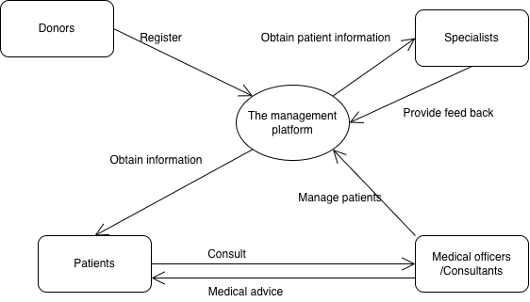
\includegraphics[width=0.8\textwidth]{images/context.png}	
\end{center}
\caption{Context Diagram}
\label{fig:context}
\end{figure}

\newpage

\subsection{Architecture Design}
Architectural Design shows the major components of a system and depicts the interconnectivity between each of them. The properties and interfaces are shown. The internal details specific to each component are ignored in the process.  

\begin{figure}[h]
\begin{center}
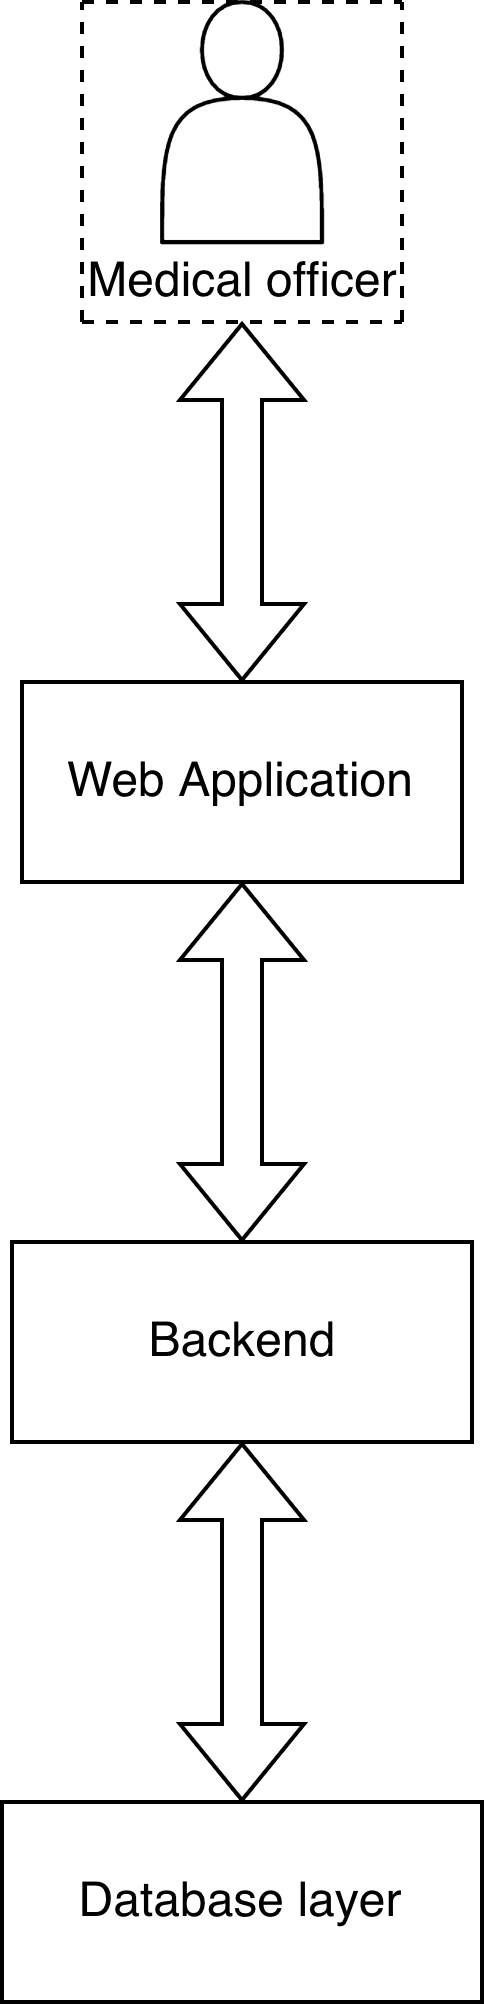
\includegraphics[width=0.2\textwidth]{images/arch.png}	
\end{center}
\caption{Architecture Diagram}
\label{fig:arch}
\end{figure}


\subsection{Detailed Design}
The detailed design of the system consists of ER Diagrams, Activity Diagrams, and Sequence diagrams primarily. Entity Relationship Diagram shows most of the internal data structures relevant to the system. It also shows the relationship of the objects situated within the system.

\subsubsection*{Entity Relationship Diagram}

Figure \ref{fig:er} shows the entity-relationship diagram of the system. The system uses a sequential ID for users.

\begin{figure}[h]
\begin{center}
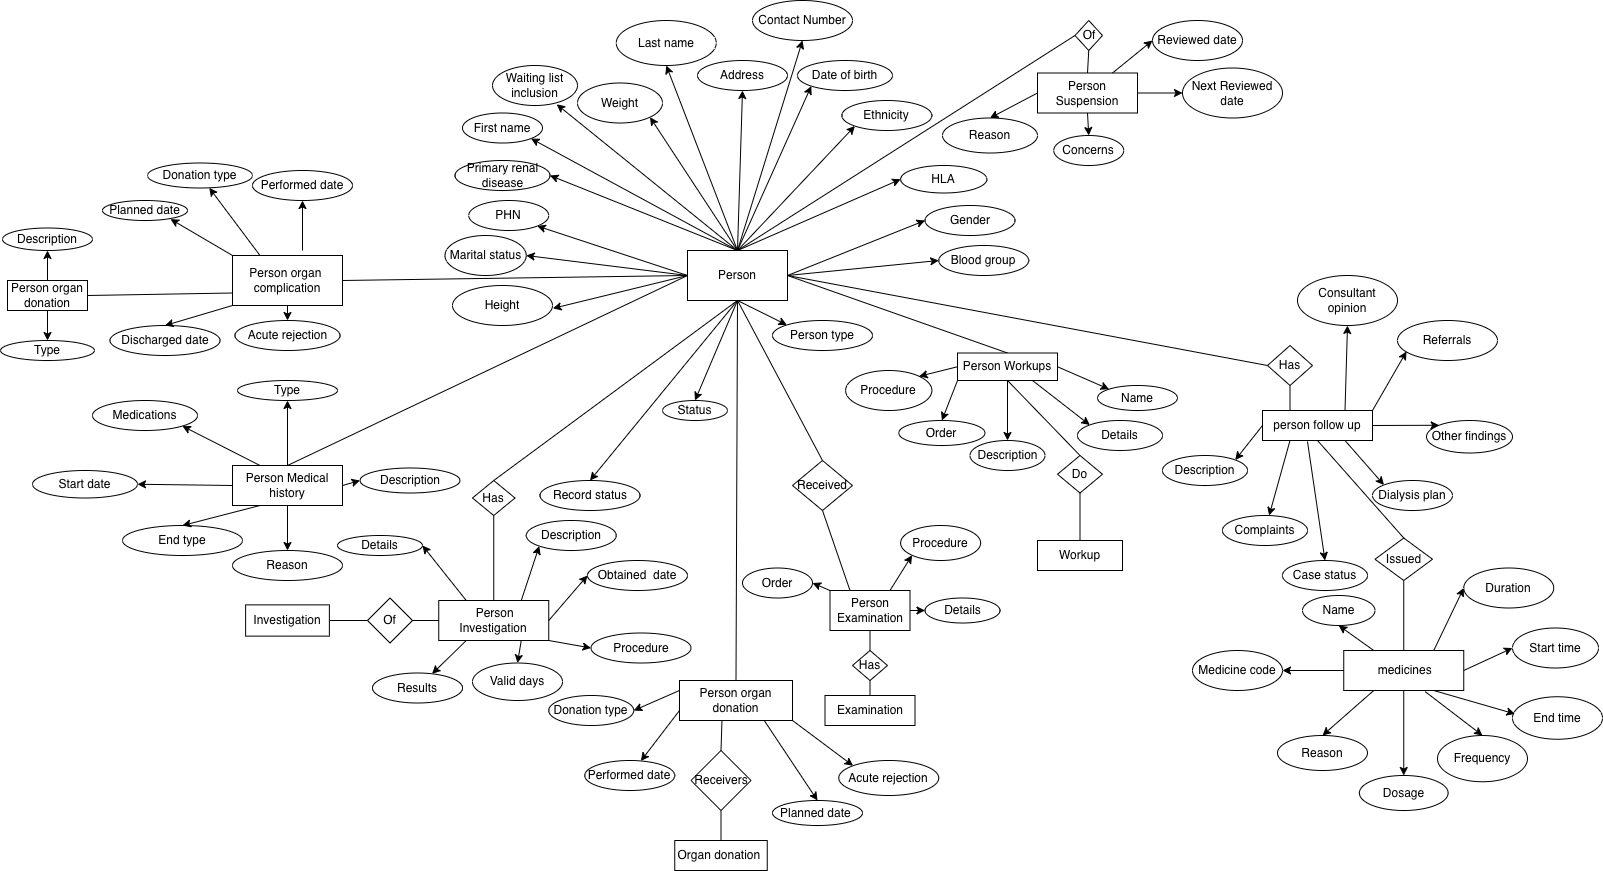
\includegraphics[width=\textwidth]{images/er.png}	
\end{center}
\caption{ER Diagram}
\label{fig:er}
\end{figure}




\newpage 

Figure \ref{fig:usecase} depicts the interaction of the system with outside \& internal components. 
 \begin{figure}[hbp]
\begin{center}
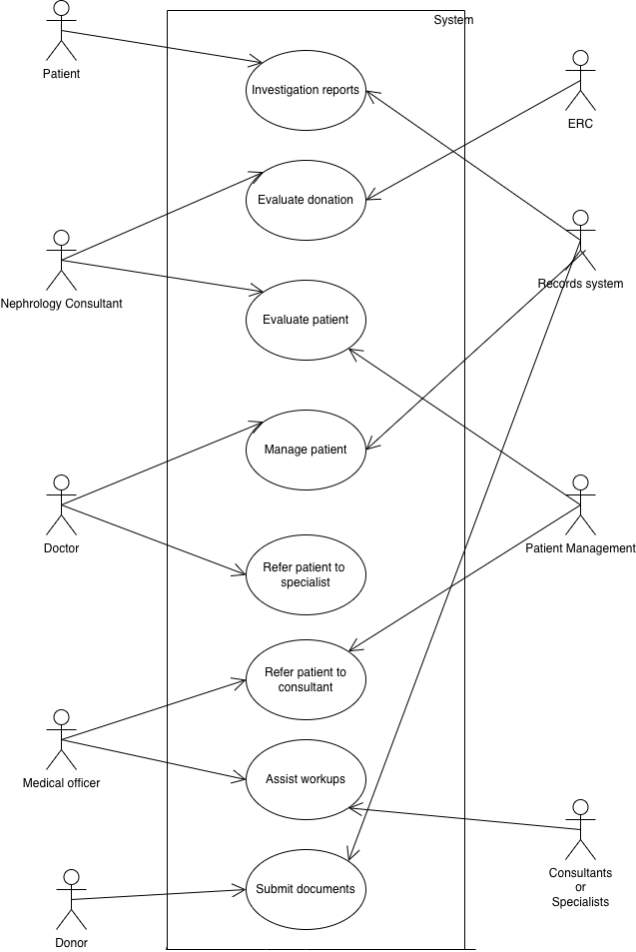
\includegraphics[width=0.75\textwidth]{images/high-level-usecase.png}	
\end{center}
\caption{High-level Usecase Diagram of the proposed system}
\label{fig:usecase}
\end{figure}


 

 
 
\newpage


 \begin{figure}[hbp]
\begin{center}
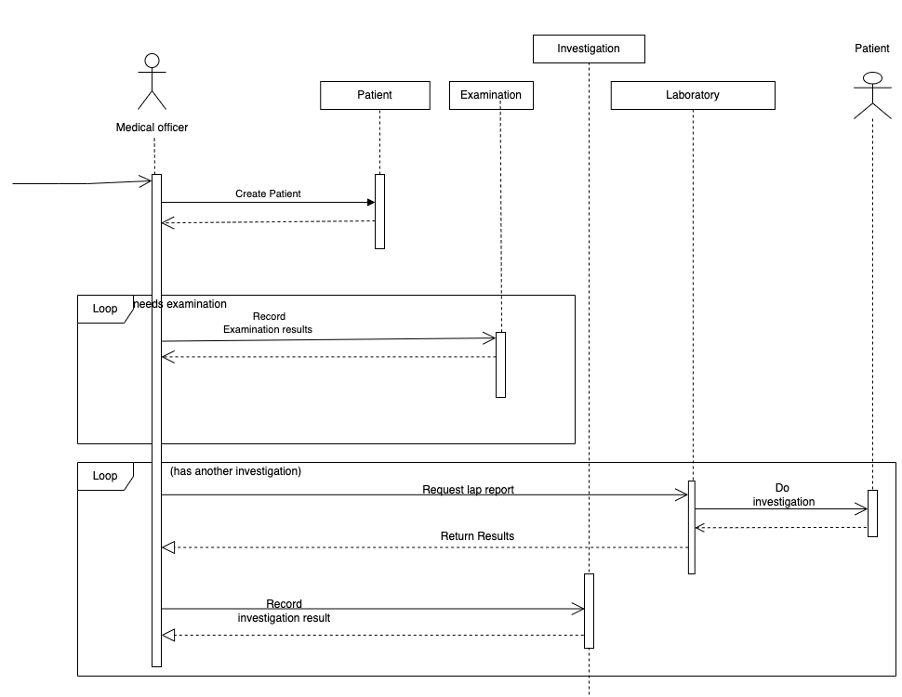
\includegraphics[width=\textwidth]{images/patient-registration.png}	
\end{center}
\caption{Sequence Diagram for Patient Registration}
\label{fig:patient-registration}
\end{figure}


Figure \ref{fig:patient-registration} depicts the flow during which a new patient is added to the system. There are multiple steps involved in the process. 
 
 
\newpage 
 
 \begin{figure}[hbp]
\begin{center}
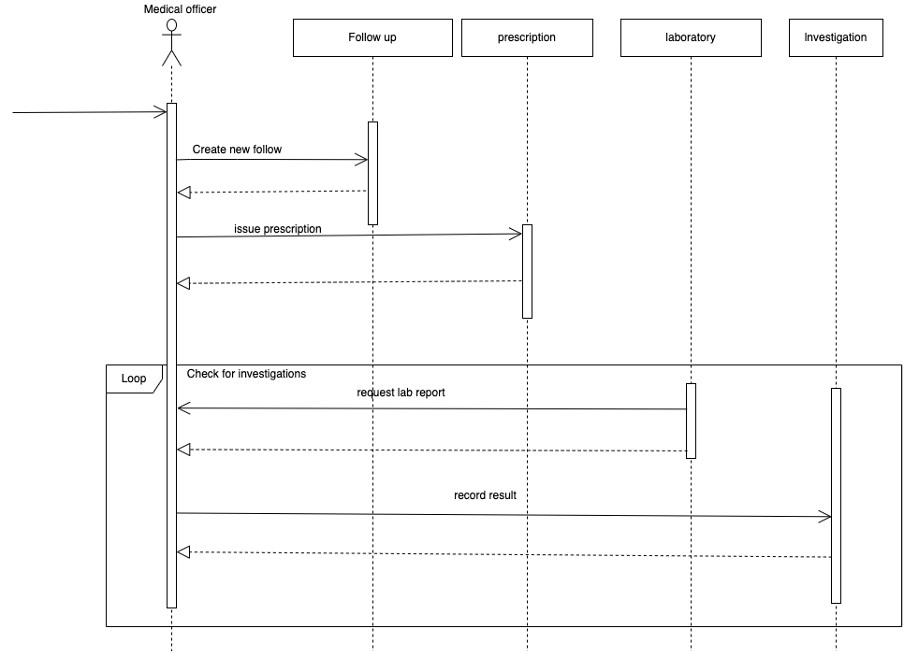
\includegraphics[width=\textwidth]{images/followups.png}	
\end{center}
\caption{Sequence Diagram for Follow Ups}
\label{fig:patient-followups}
\end{figure}

Figure \ref{fig:patient-followups} shows the follow-up procedure in the hospital.  The patients are usually followed up on their regular clinic visits. The follow-up sequences are currently followed up in the clinic books but will be digitized in the new system.

\newpage
 
 \begin{figure}[hbp]
\begin{center}
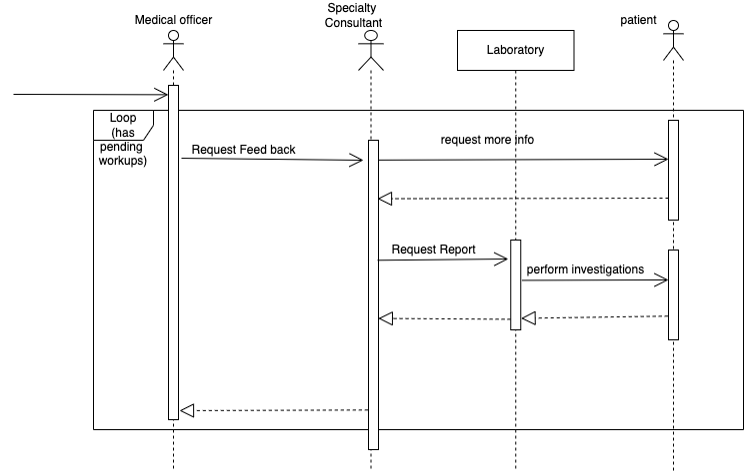
\includegraphics[width=\textwidth]{images/workups.png}	
\end{center}
\caption{Sequence Diagram for Workups}
\label{fig:patient-workups}
\end{figure}
Once the patient completes the necessary registration and passes the Kidney Transplant checklist, the patient is enrolled for workups. The workups are repeated until the patient has gone through all the Specialist doctors referred. Figure \ref{fig:patient-workups} shows the sequence diagram for workups.



\newpage
 

 \begin{figure}[hbp]
\begin{center}
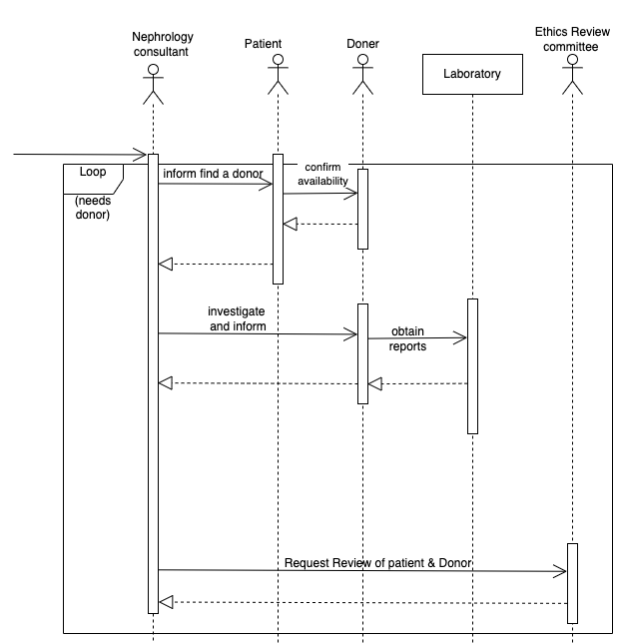
\includegraphics[width=\textwidth]{images/donor-finding.png}	
\end{center}
\caption{Donor Finding}
\label{fig:donor-finding}
\end{figure}
The donors can be found by a Patient on their own if they need a kidney transplant. The donor needs to be fully informed of the decision and they need to go through similar steps of workups and investigations before they are allowed to go ahead with the surgery. In this manner, the donor is thoroughly reviewed. Figure \ref{fig:donor-finding} shows the procedure followed in Donor Finding. 

\chapter{Implementation}
The implementation phase is crucial in the software's lifecycle. The system is developed during this phase, according to the details gathered in the previous stages. It requires a significant amount of time to complete. The outcome of the implementation phase is deliverable. The deliverable should satisfy the requirements of the client and improve their work processes.

\section{Implementation Environment}

Software development has specific requirements for every product. Such that the implementation environment must be specified for the development. The system should be able to cater to the demand of the users as well. Following are the minimum hardware requirements for the project to successfully cater to 100 simultaneous users and store details for up to 1 year for 5000 patients.

The Application Server requires two parallel servers operating to obtain a highly available environment and to do rolling updates. 

Hardware Requirements for Application Server: (2 Servers)
\begin{itemize}
	\item 2.5GHz (4-core CPU)
	\item 4GB RAM
	\item 50GB SSD
\end{itemize}

Hardware Requirements for Database Server: (1 Server)
\begin{itemize}
	\item 2.5GHz (4-core CPU)
	\item 4GB RAM
	\item 500GB SSD
\end{itemize}

In addition to the above requirements, in order to access the system users will require a computer running Google Chrome / Webkit browser released after 2018 for better performance gains. The system processes most of the data on the server. Hence it should work fine for most computers with an internet browser released later than 2017.

\subsection*{Technical Specifications}
\begin{itemize}
	\item Database Layer: PostgresDB
	\item Application Layer: Single binary file built from Golang
\end{itemize}

\section{Development Environment}

\subsection*{Hardware}

\begin{itemize}
	\item 2.5GHz-octa-core CPU (All-in-one Database, Application)
	\item 16GB RAM
	\item 10GB Storage
\end{itemize}
\subsection*{Software}
\begin{itemize}
\item macOS
\item Jetbrains Intellij Idea 2022.1
\item Golang 1.18
\item PostgreSQL 14
\end{itemize}


\newpage 
\section{Code / Module Architecture}
Golang was chosen for the implementation of the backend. The latest version of 1.18 was used to develop the system since it provides some additional features like Generics. The backend is architected on top of a Golang framework called Beego. An extensible GraphQL Specification is implemented using a GraphQL Library called "GqlGen" which is available in Golang. The specification allows the system to be extensible without making many changes on the front end. 

The system has been implemented with a custom Role-Based Access Control (RBAC). It allows different types of users to be assigned different permissions in the future as well. The permissions are predefined in the GraphQL Schema, which can be altered to ensure access control policies are sufficient.

The components of the system are as follows

\begin{itemize}
	\item Users Management - Interface for managing access for the users and their permissions
	\item Patients Management - Interface for managing patients, includes components such as investigations, examinations, etc.
	\item Workflow Management - Interface for managing any customized workflow pertaining to their job role.

\end{itemize}


\chapter{Evaluation}

The evaluation process in a software development life cycle is carried out to ensure that the system satisfies the user requirements. In this phase, the user requirements are verified to be available in the system. The system has to be tested with Sample data. This ensures that the features developed are free of issues, which is crucial for the successful delivery of a software system. Hence testing part should be done with full consideration of the features.

\section{Testing Procedure}
The system can be tested for issues in multiple manners. The testing procedures usually start from the Unit Level for each and every function and proceed up. Integration testing for each and every component ensures that the functionality is as expected when the components are working together. The system testing is carried out at the system level to ensure all of the components are functioning as intended. The system was allowed to be tested by the end-users to their satisfaction.

\subsection*{Unit Testing}

Golang's built-in testing toolkit has been used for Unit testing.

\subsection*{User Acceptance Testing}

These tests emulate real-world requirements and provide an environment for the software to be tested in real conditions. Hence it provides insight into how the system might perform under certain conditions. The following tests separated per module have been designed for the purpose.

\subsubsection*{Authentication and Authorization Tests}

\renewcommand{\cellalign}{l}

\begin{table}[h]
%\resizebox{\textwidth}{!}{
\begin{tabular}{|l|l|l|l|}
\hline
 \textbf{\#} & \textbf{Description}  & \textbf{Steps to Test}  & \textbf{Expected Result}   \\ \hline
1 
& 
\makecell{
Log in without\\ a Password
}
& 
\makecell{
1. Visit /auth/login\\
2. Fill in a valid username\\
3. Click Login 
}
& 
Cannot log in to the system \\ \hline



2
& 
\makecell{
Log in with \\a wrong password
}
& 
\makecell{
1. Visit /auth/login\\
2. Fill in a valid username\\
3. Fill in an invalid password\\
4. Click Login 
}
& 
Cannot log in to the system \\ \hline



3 
&
\makecell{
 Log in with \\a correct password
 }
& 
\makecell{
1. Visit /auth/login\\
2. Fill in valid username\\
3. Fill in correct password \\
4. Click Login 
}
& 
Logged in successfully \\ \hline


4 
&
Admin Access
& 
\makecell {
1. Visit the /auth/login and \\ valid admin credentials \\
2. Access Dashboard via /
}
&
\makecell {Admin Dashboard Panel \\ accessible.} \\ \hline

%5 &
%\makecell{
% 
%} 
%&
%\makecell{
%}
%&
%\makecell{
%}  \\ \hline

\end{tabular}
%}
\centering
\caption{Authentication and Authorization Tests}
\end{table}




\subsubsection*{Patient Record Access}
\renewcommand{\cellalign}{l}
\begin{table}[h]
\begin{tabular}{|l|l|l|l|}
\hline
 \textbf{\#} & \textbf{Description}  & \textbf{Steps to Test}  & \textbf{Expected Result}   \\ \hline
1 &
\makecell{
Add a new Patient \\ to the system
} 
&
\makecell{
1. Login as a Consultant / Doctor \\
2. Click Patients list view \\
3. Click <New> on Top-bar \\
}
&
\makecell{
Add Patient view visible
}  \\ \hline


2 &
\makecell{
View Patient History
} 
&
\makecell{
1. Login as a Consultant / Doctor \\
2. Click Patients list view \\
3. Click View on a Patient \\
4. Open the History Tab
}
&
\makecell{
 The recorded medical\\ history of the\\ patient is visible
}  \\ \hline


3 &
\makecell{
Record a new consultation
} 
&
\makecell{
1. Login as a Consultant / Doctor \\
2. Click Patients list view \\
3. Click View on a Patient \\
4. Open the new Follow up tab \\
5. Fill Details \& Save
}
&
\makecell{
New Follow Up Form\\ visible  \& Saveable
}  \\ \hline



3 &
\makecell{
Record a new examination
} 
&
\makecell{
1. Login as a Consultant / Doctor \\
2. Click Patients list view \\
3. Click View on a Patient \\
4. Open the new Examination tab \\
}
&
\makecell{
New Examination \\Form visible
}  \\ \hline



\end{tabular}
\centering
\caption{Patient Record Access}
\end{table}
 
\newpage


\subsubsection*{Workflow Management}
\renewcommand{\cellalign}{l}
\begin{table}[h]
\begin{tabular}{|l|l|l|l|}
\hline
 \textbf{\#} & \textbf{Description}  & \textbf{Steps to Test}  & \textbf{Expected Result}   \\ \hline


1 &
\makecell{
Create new workflow
} 
&
\makecell{
1. Log in as a Consultant/Doctor \\
2. Visit Dashboard \\
3. Click "Workflows" on \\Sidebar \\
4. Click "New" on Topbar \\
}
&
\makecell{
New Workflow Creation
}  \\ \hline



2 &
\makecell{
Use Workflow
} 
&
\makecell{
1. Log in as a Consultant/Doctor \\
2. Open a patient record \\
3. Click a workflow in \\ the right sidebar\\
4. Process the workflow\\
}
&
\makecell{
Patient record presented \\ 
according to the workflow \\
and allows input to me made
}  \\ \hline



\end{tabular}
\centering
\caption{Workflow Management}
\end{table}


%\subsubsection*{}
%\renewcommand{\cellalign}{l}
%\begin{table}[h]
%\begin{tabular}{|l|l|l|l|}
%\hline
% \textbf{\#} & \textbf{Description}  & \textbf{Steps to Test}  & \textbf{Expected Result}   \\ \hline
%5 &
%\makecell{
%} 
%&
%\makecell{
%}
%&
%\makecell{
%}  \\ \hline
%\end{tabular}
%\centering
%\caption{}
%\end{table}


%\subsubsection*{}
%\renewcommand{\cellalign}{l}
%\begin{table}[h]
%\begin{tabular}{|l|l|l|l|}
%\hline
% \textbf{\#} & \textbf{Description}  & \textbf{Steps to Test}  & \textbf{Expected Result}   \\ \hline
%5 &
%\makecell{
%} 
%&
%\makecell{
%}
%&
%\makecell{
%}  \\ \hline
%\end{tabular}
%\centering
%\caption{}
%\end{table}


\chapter{Conclusion}

The project was successfully completed to achieve the scope which was determined during the design period as critical components. The client’s User Acceptance Testing was conducted to ensure that client's fundamental requirements are met to use the system.

\section{Lessons Learnt}

The development of the platform resulted in great experience in developing GraphQL-based technology. It expanded knowledge and the technical know-how of project management principles. 

\section{Future work}

Implementing more robust controls on the setup to record historic values of patients' health. 
Implementation of a mobile application for easier access. 



\appendix
\addcontentsline{toc}{chapter}{Appendices}
\chapter{System Manual}

Figure \ref{fig:dirlayout} shows the layout of the application. \\ 

In the root of the directory, Golang binary is built and run using the command "go build -o backend" 

Within the "frontend" directory, the dependencies of the frontend has to be installed before building it. It can be installed by using "npm / pnpm.io".

\begin{figure}[h]
\begin{center}
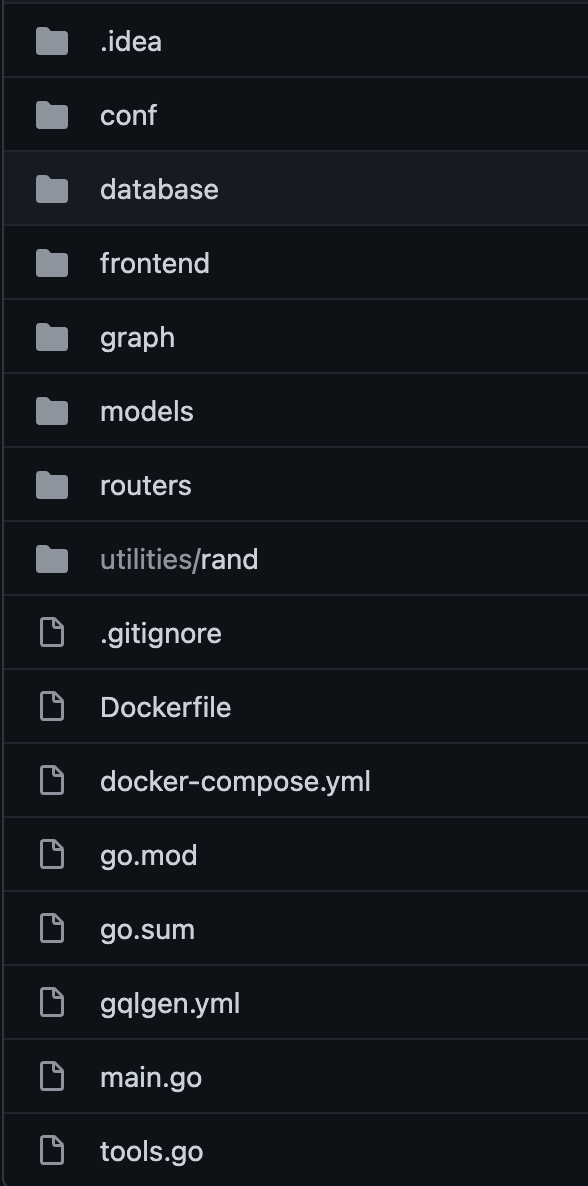
\includegraphics[width=0.8\textwidth,scale=0.25]{images/directory-layout.png}	
\end{center}
\caption{Directory Layout}
\label{fig:dirlayout}
\end{figure}
%\chapter{Design Documentation}


\chapter{User Manual}

Following Figure \ref{fig:login} shows the login screen which the user is greeted with whenever they are accessing any part of the system.
\begin{figure}[hbp]
\begin{center}
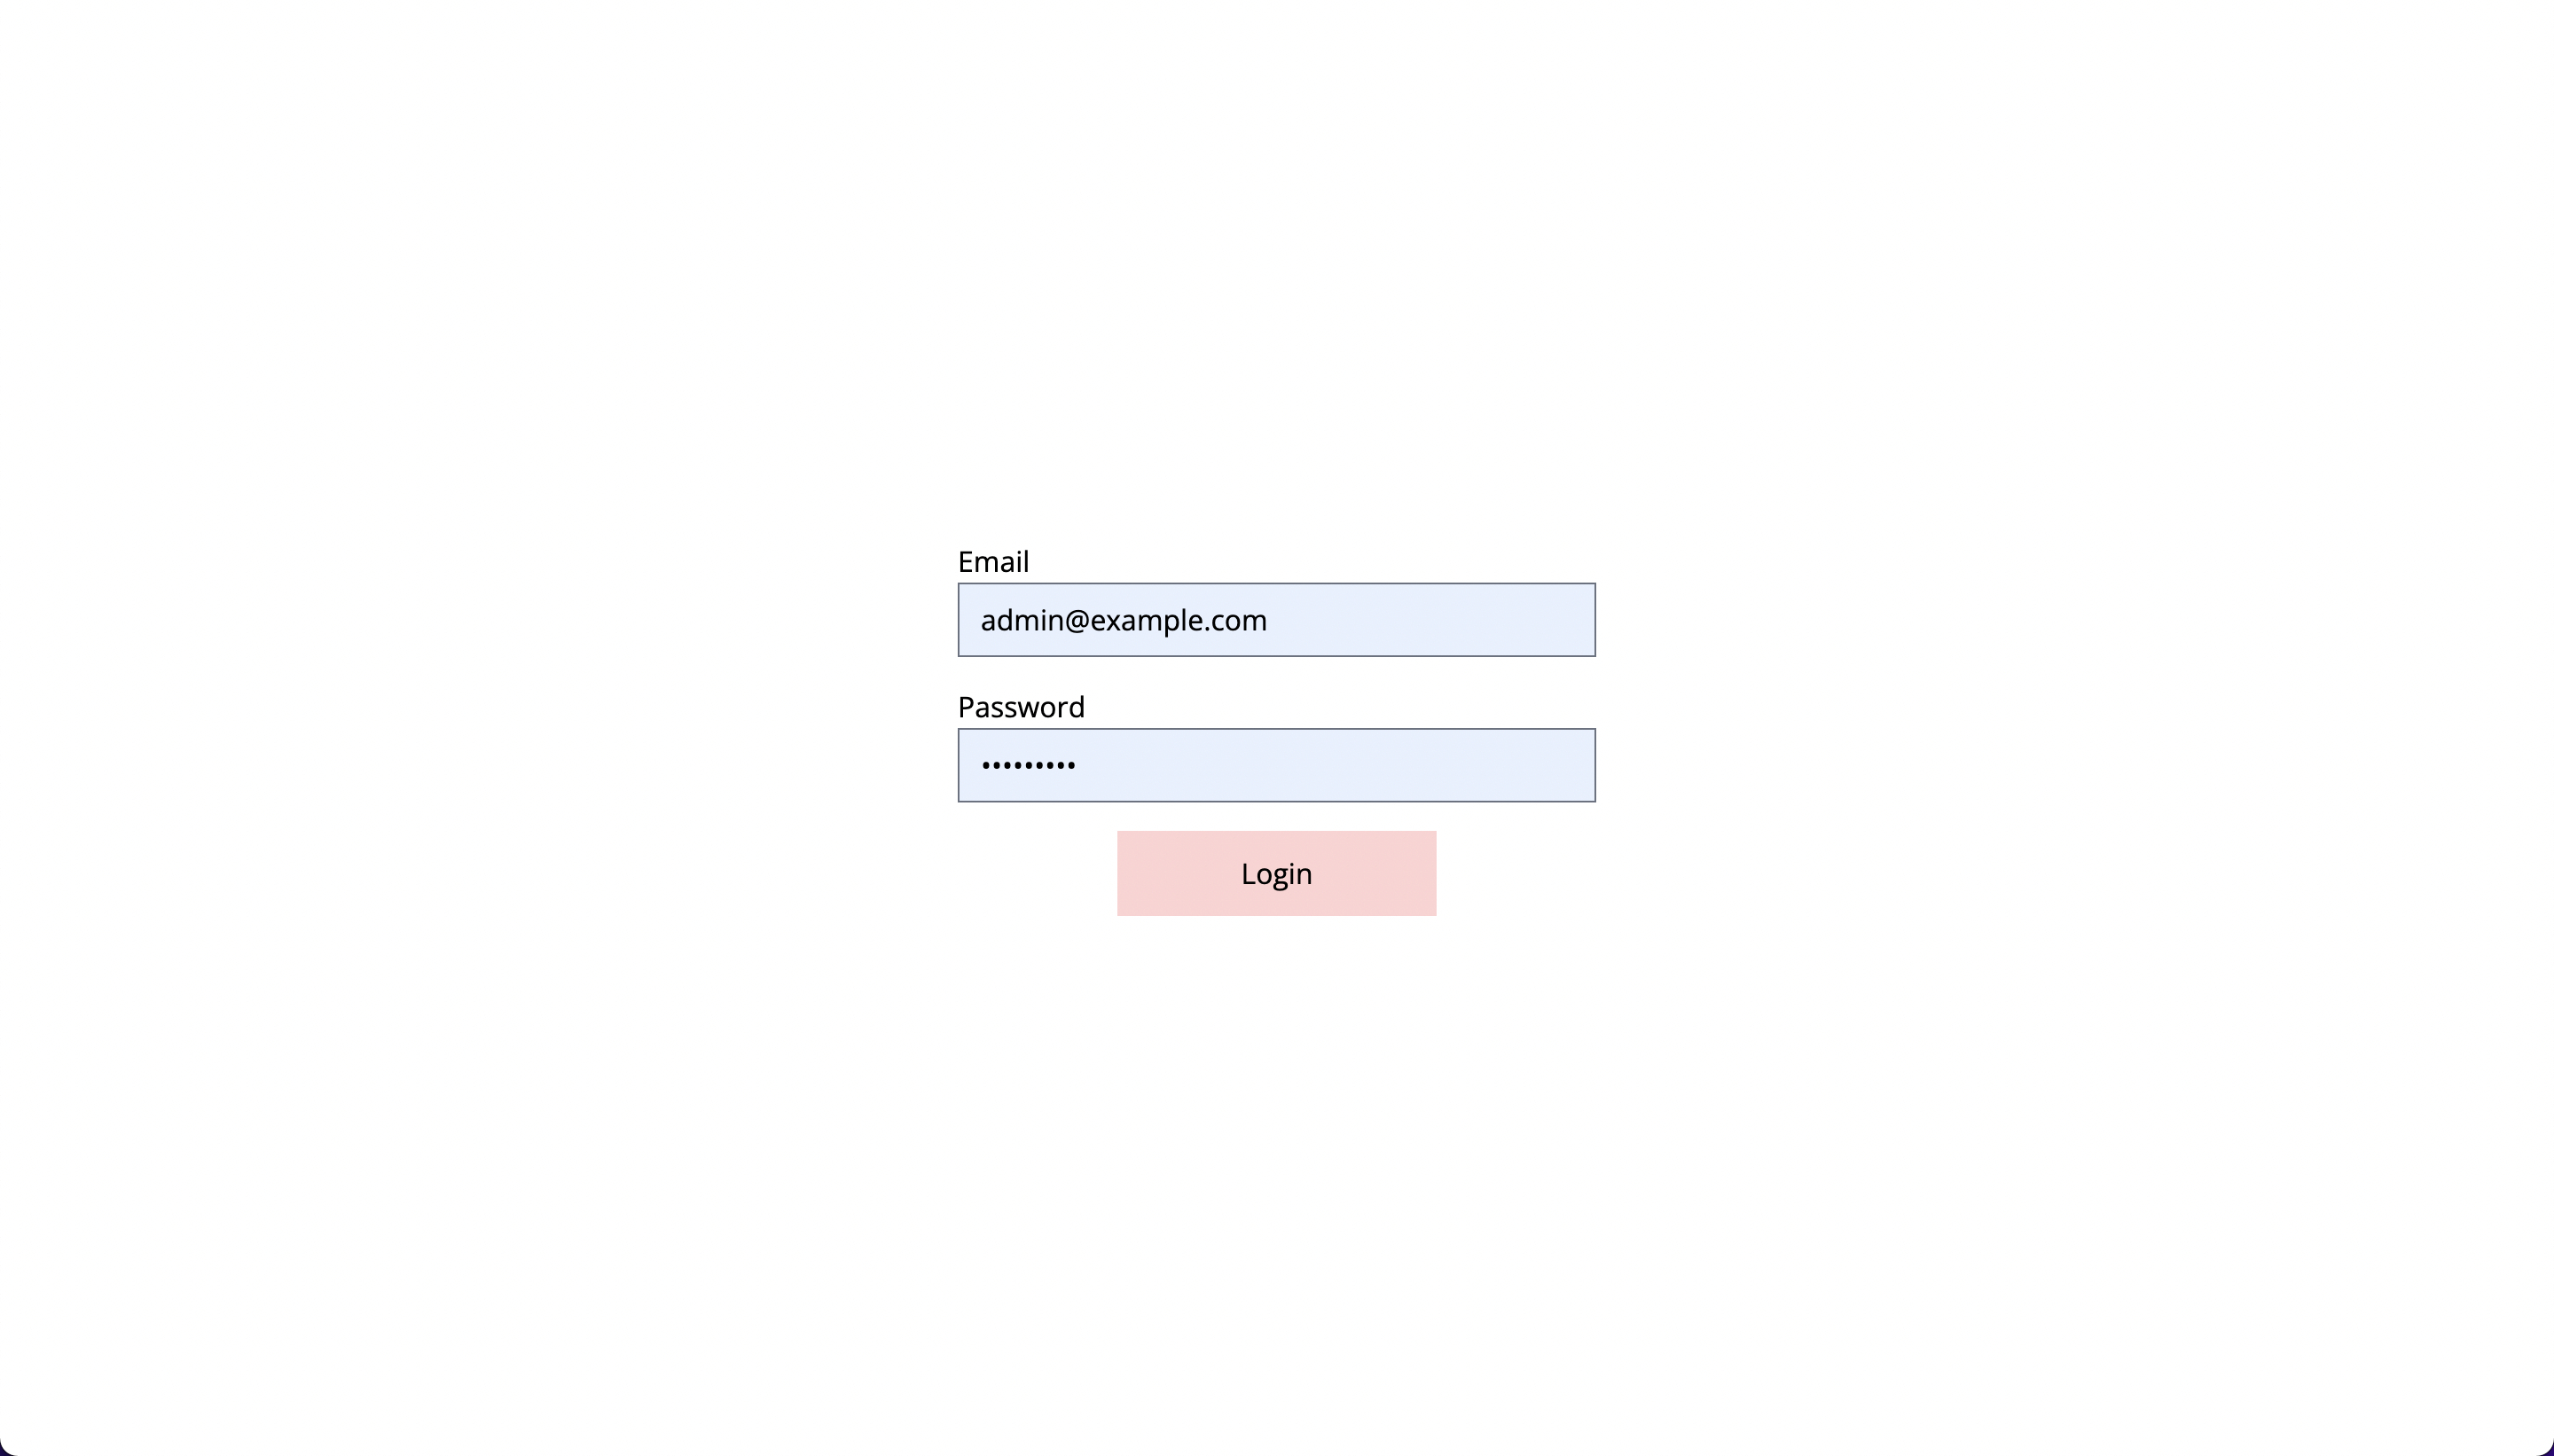
\includegraphics[width=0.8\textwidth,scale=0.25]{images/login-screen.png}	
\end{center}
\caption{Login Screen}
\label{fig:login}
\end{figure}



 
Figure \ref{fig:dashboard} shows Dashboard layout on which the user primarily lands for further actions. This layout is to be expanded with more charts in the future.

\begin{figure}[hbp]
\begin{center}
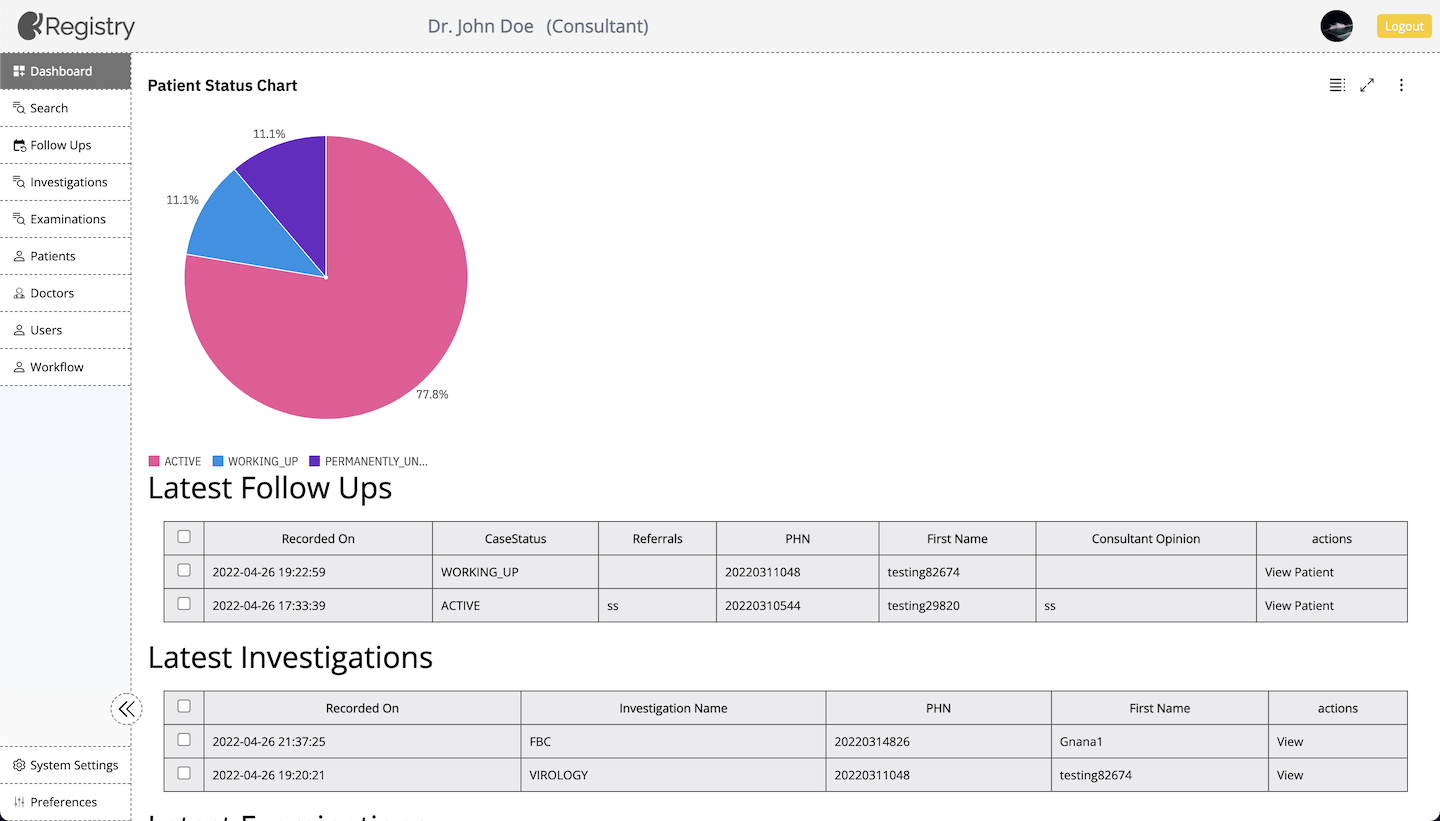
\includegraphics[width=0.8\textwidth,scale=0.25]{images/dashboard.png}	
\end{center}
\caption{Dashboard Screen}
\label{fig:dashboard}
\end{figure}



Figure \ref{fig:search-layout} shows screen that allows the user to search for patients in the system. 

\begin{figure}[hbp]
\begin{center}
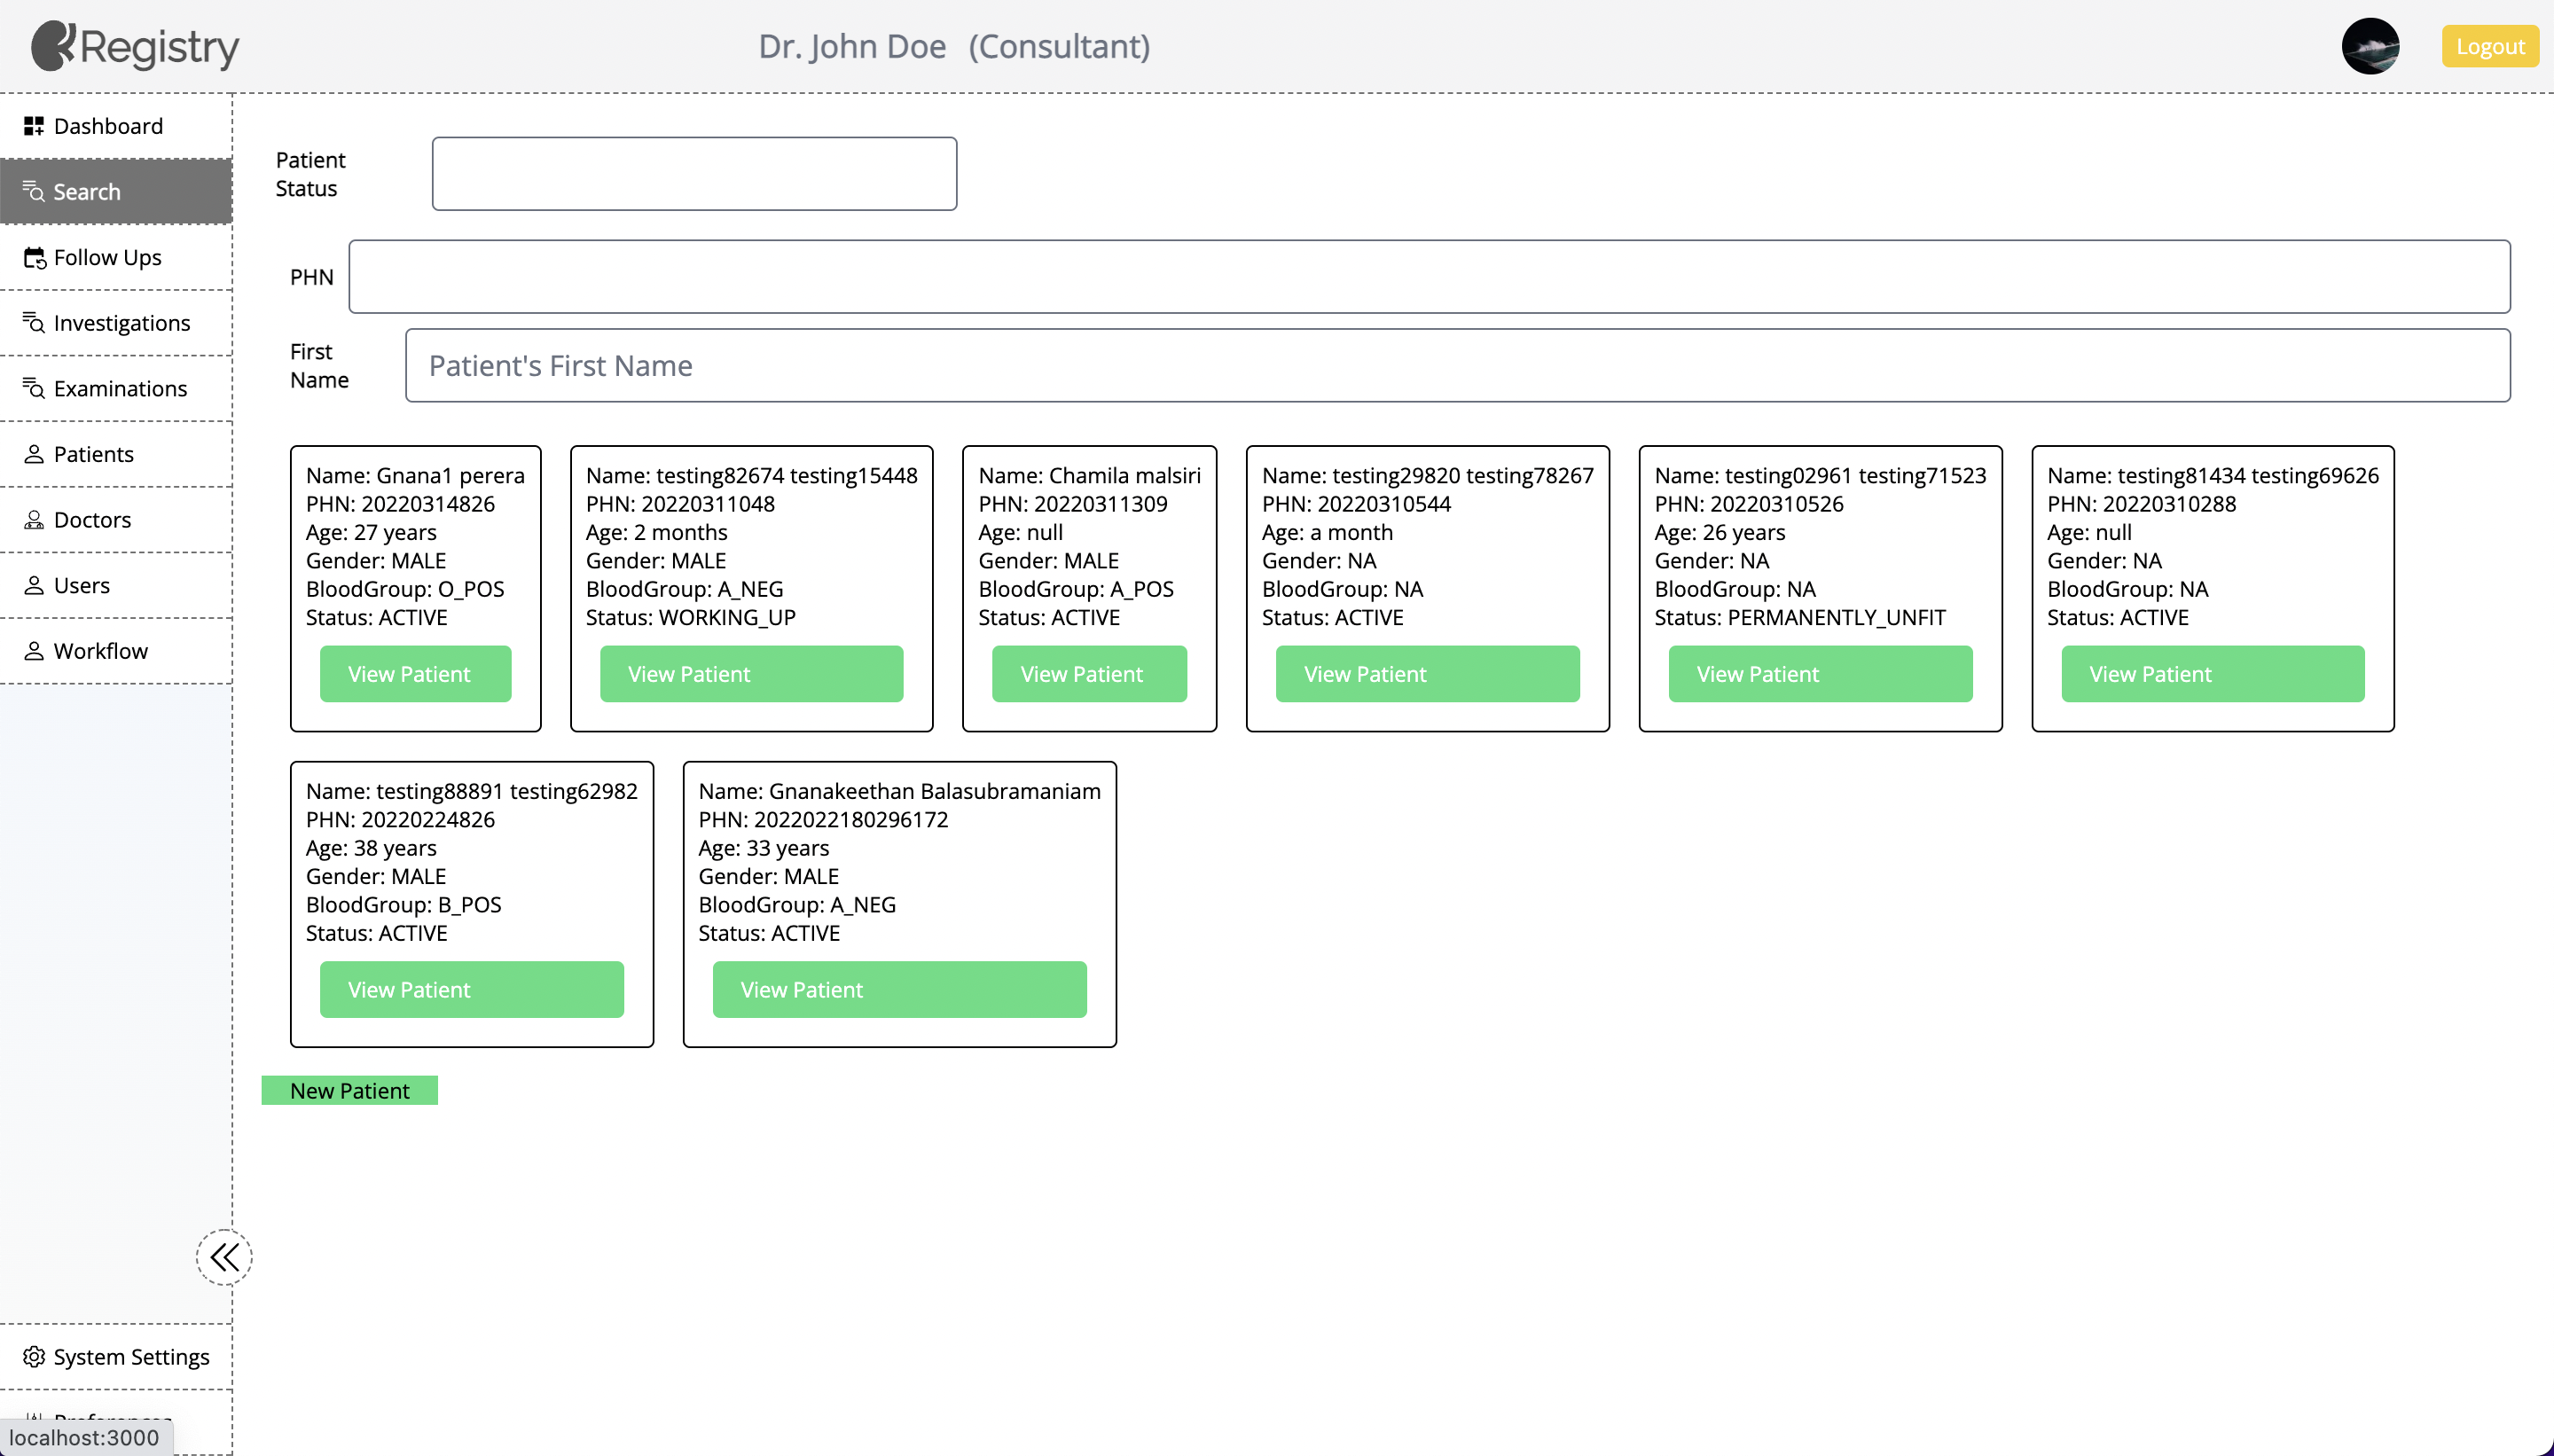
\includegraphics[width=0.8\textwidth,scale=0.25]{images/search.png}	
\end{center}
\caption{Search Patients Screen}
\label{fig:search-layout}
\end{figure}



Figure \ref{fig:patient-list} shows the list of patients in the system in a tabular manner. 


\begin{figure}[hbp]
\begin{center}
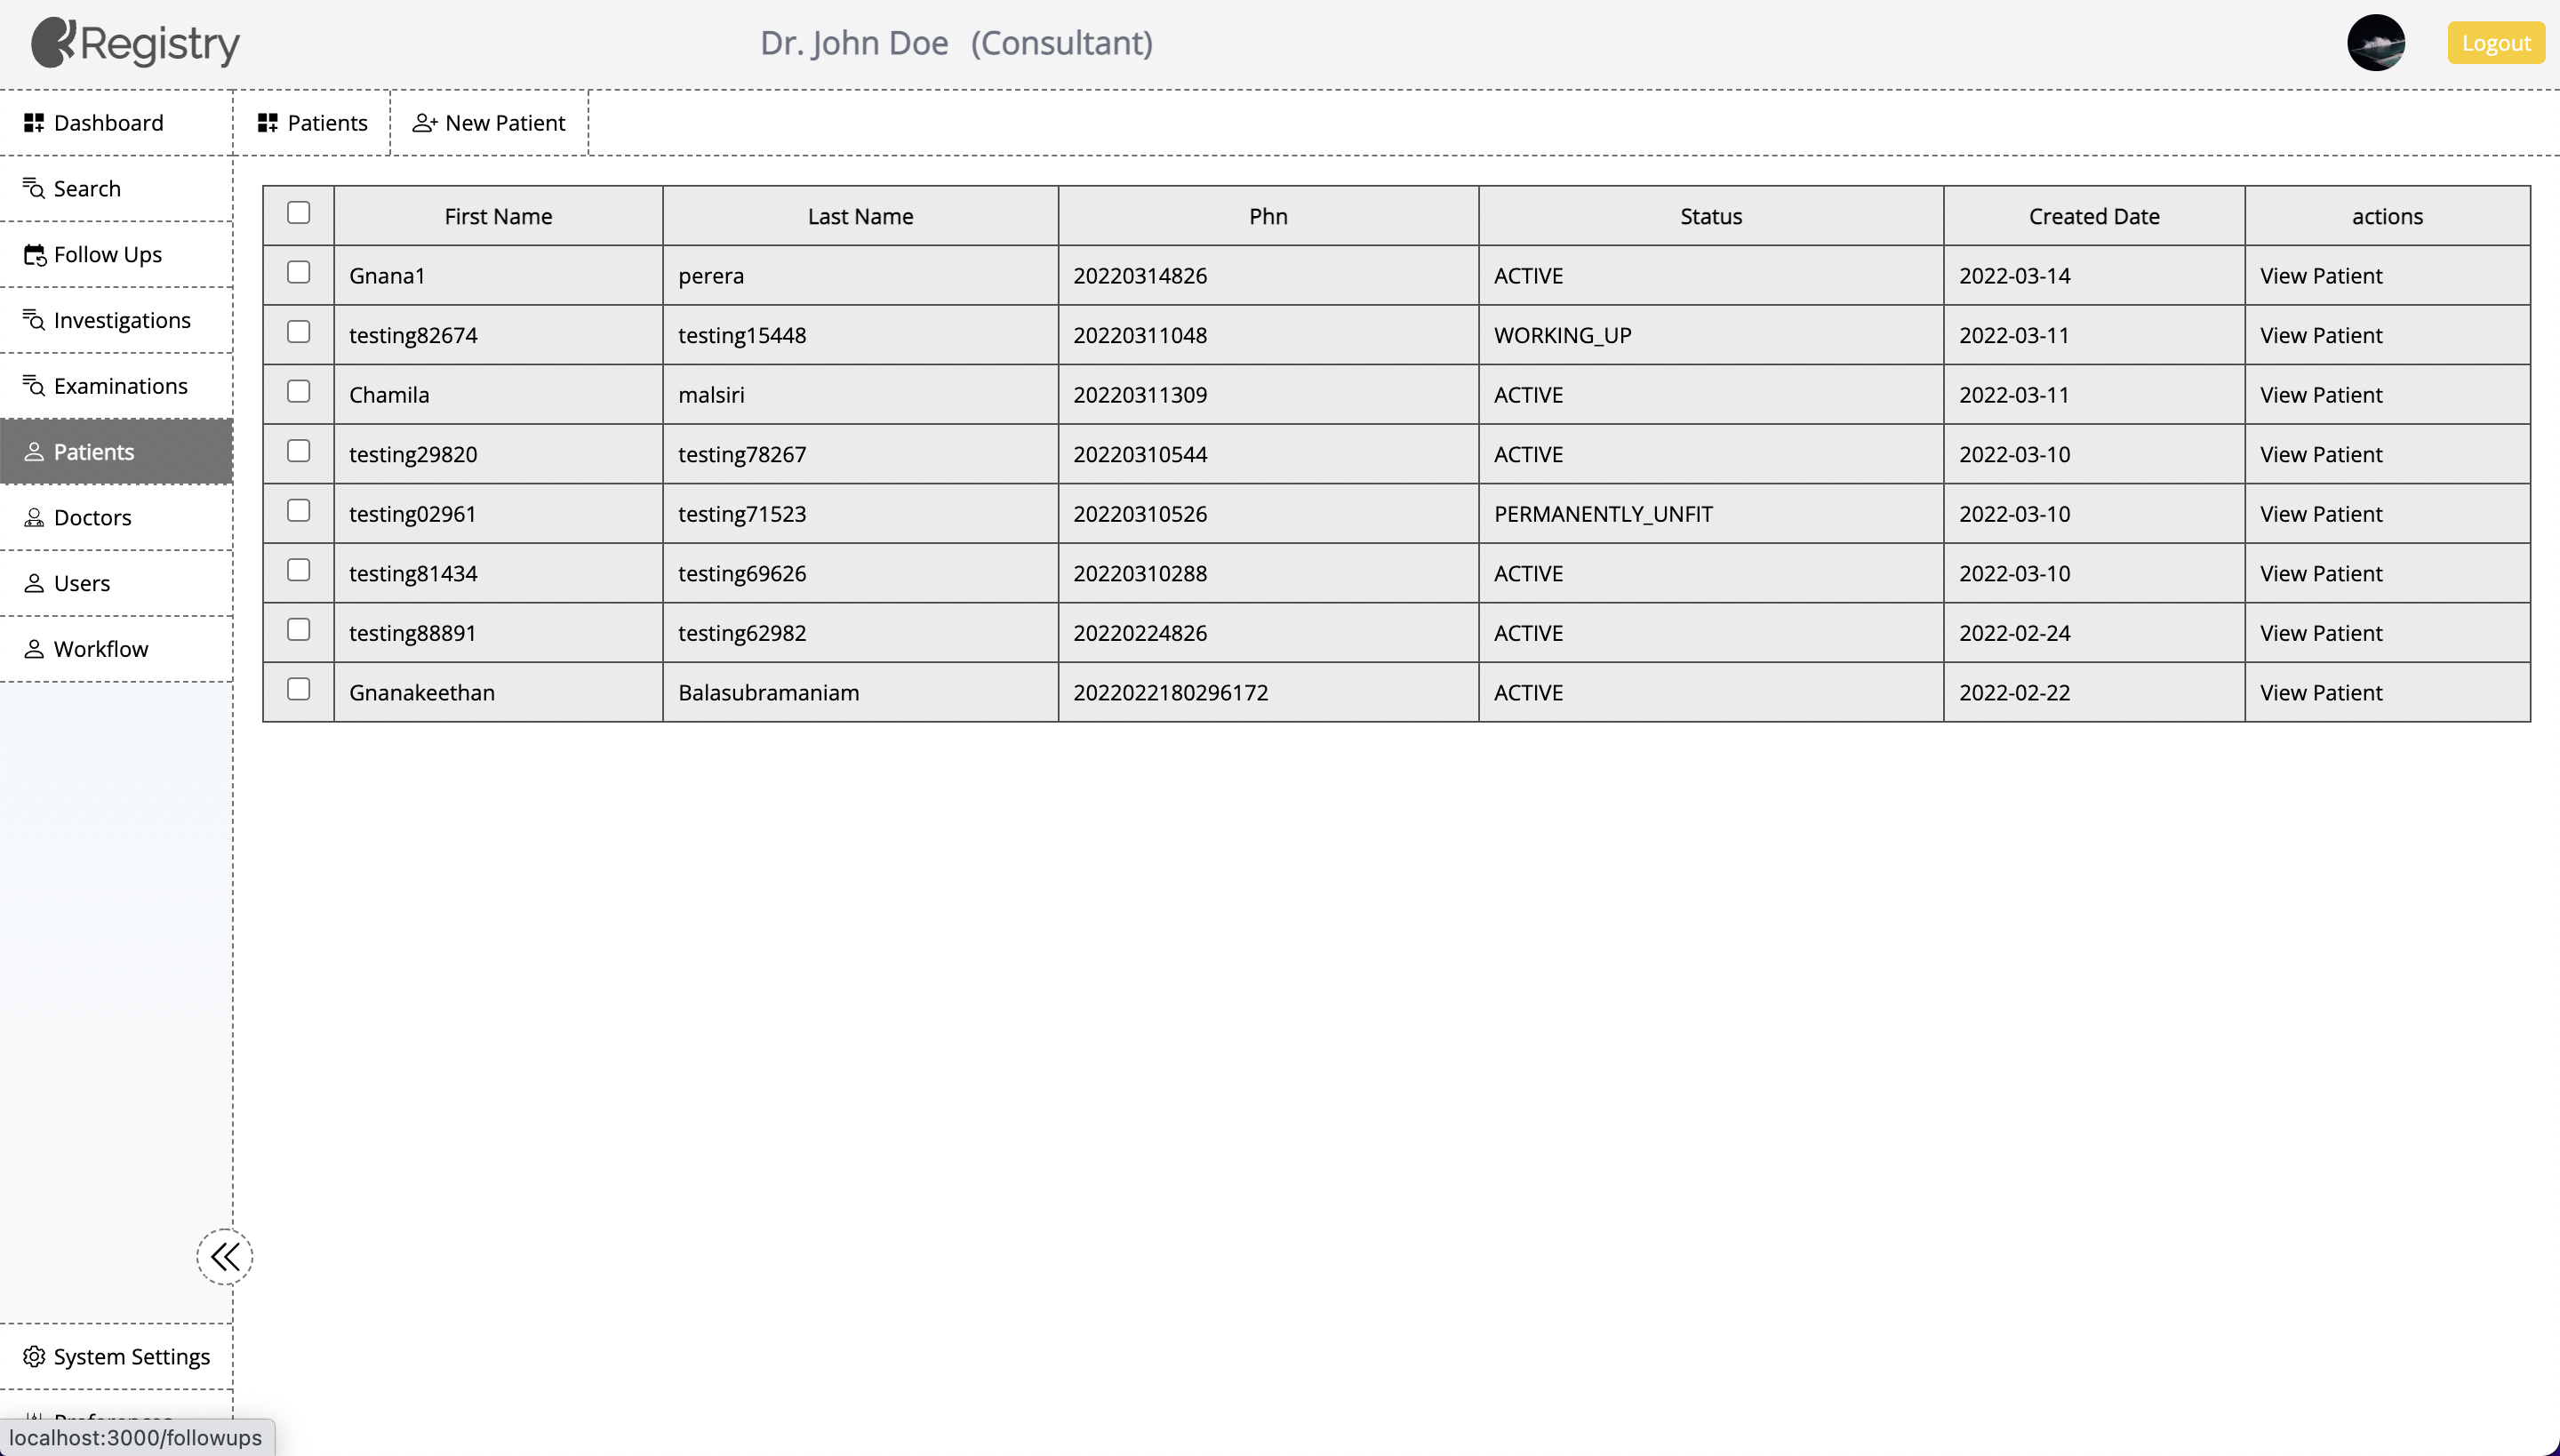
\includegraphics[width=0.8\textwidth,scale=0.25]{images/patients-list.png}	
\end{center}
\caption{List of Patients Screen}
\label{fig:patient-list}
\end{figure}




Figure \ref{fig:patient-history} shows a specific patient's historical records. 

\begin{figure}[h]
\begin{center}
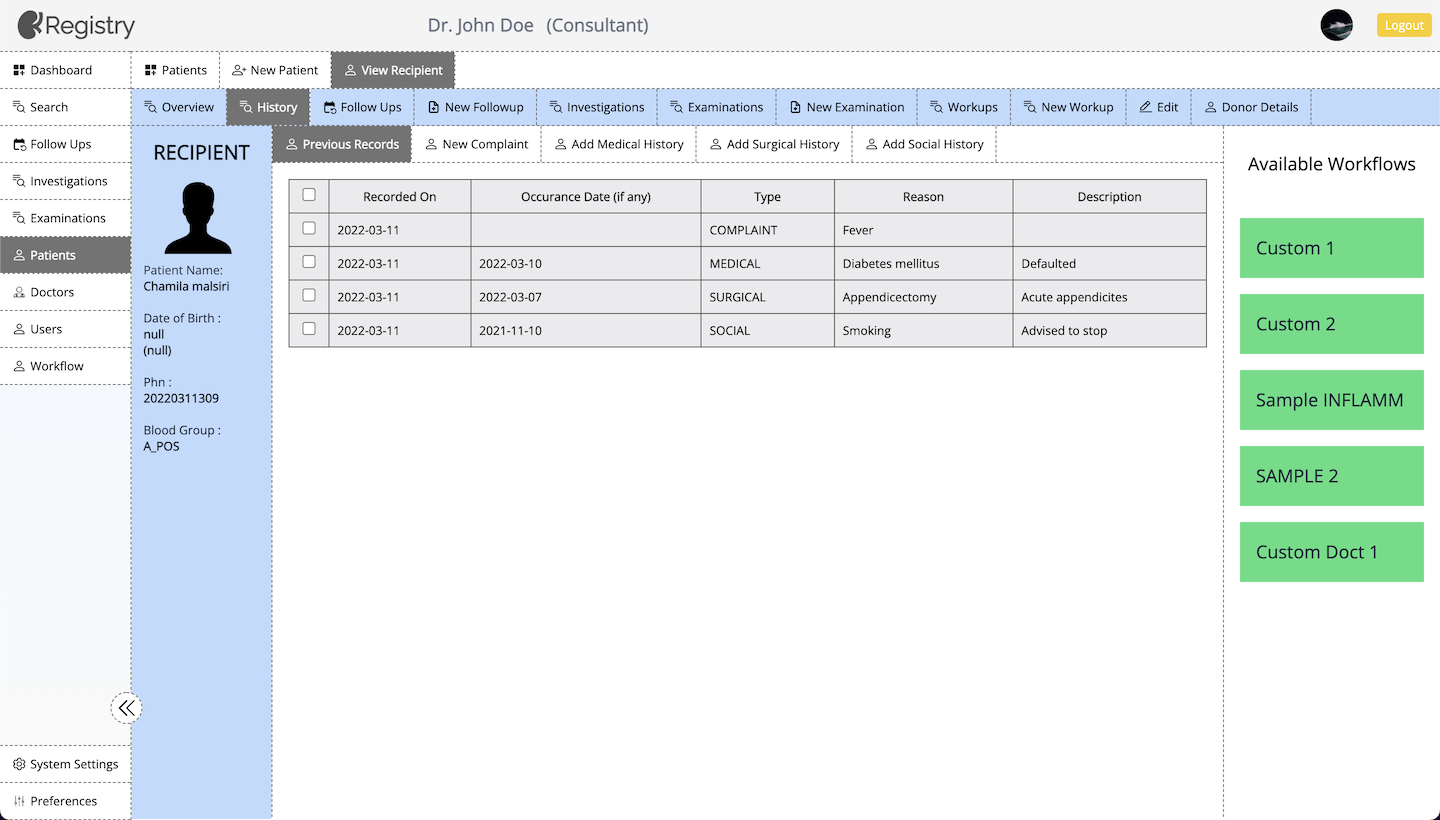
\includegraphics[width=0.8\textwidth,scale=0.25]{images/patient-history.png}	
\end{center}
\caption{Patient History Screen}
\label{fig:patient-history}
\end{figure}




%Figure \ref{fig:patient-registration-screen} shows a form for which the patient can be registered with the system.
%
%\begin{figure}[h]
%\begin{center}
%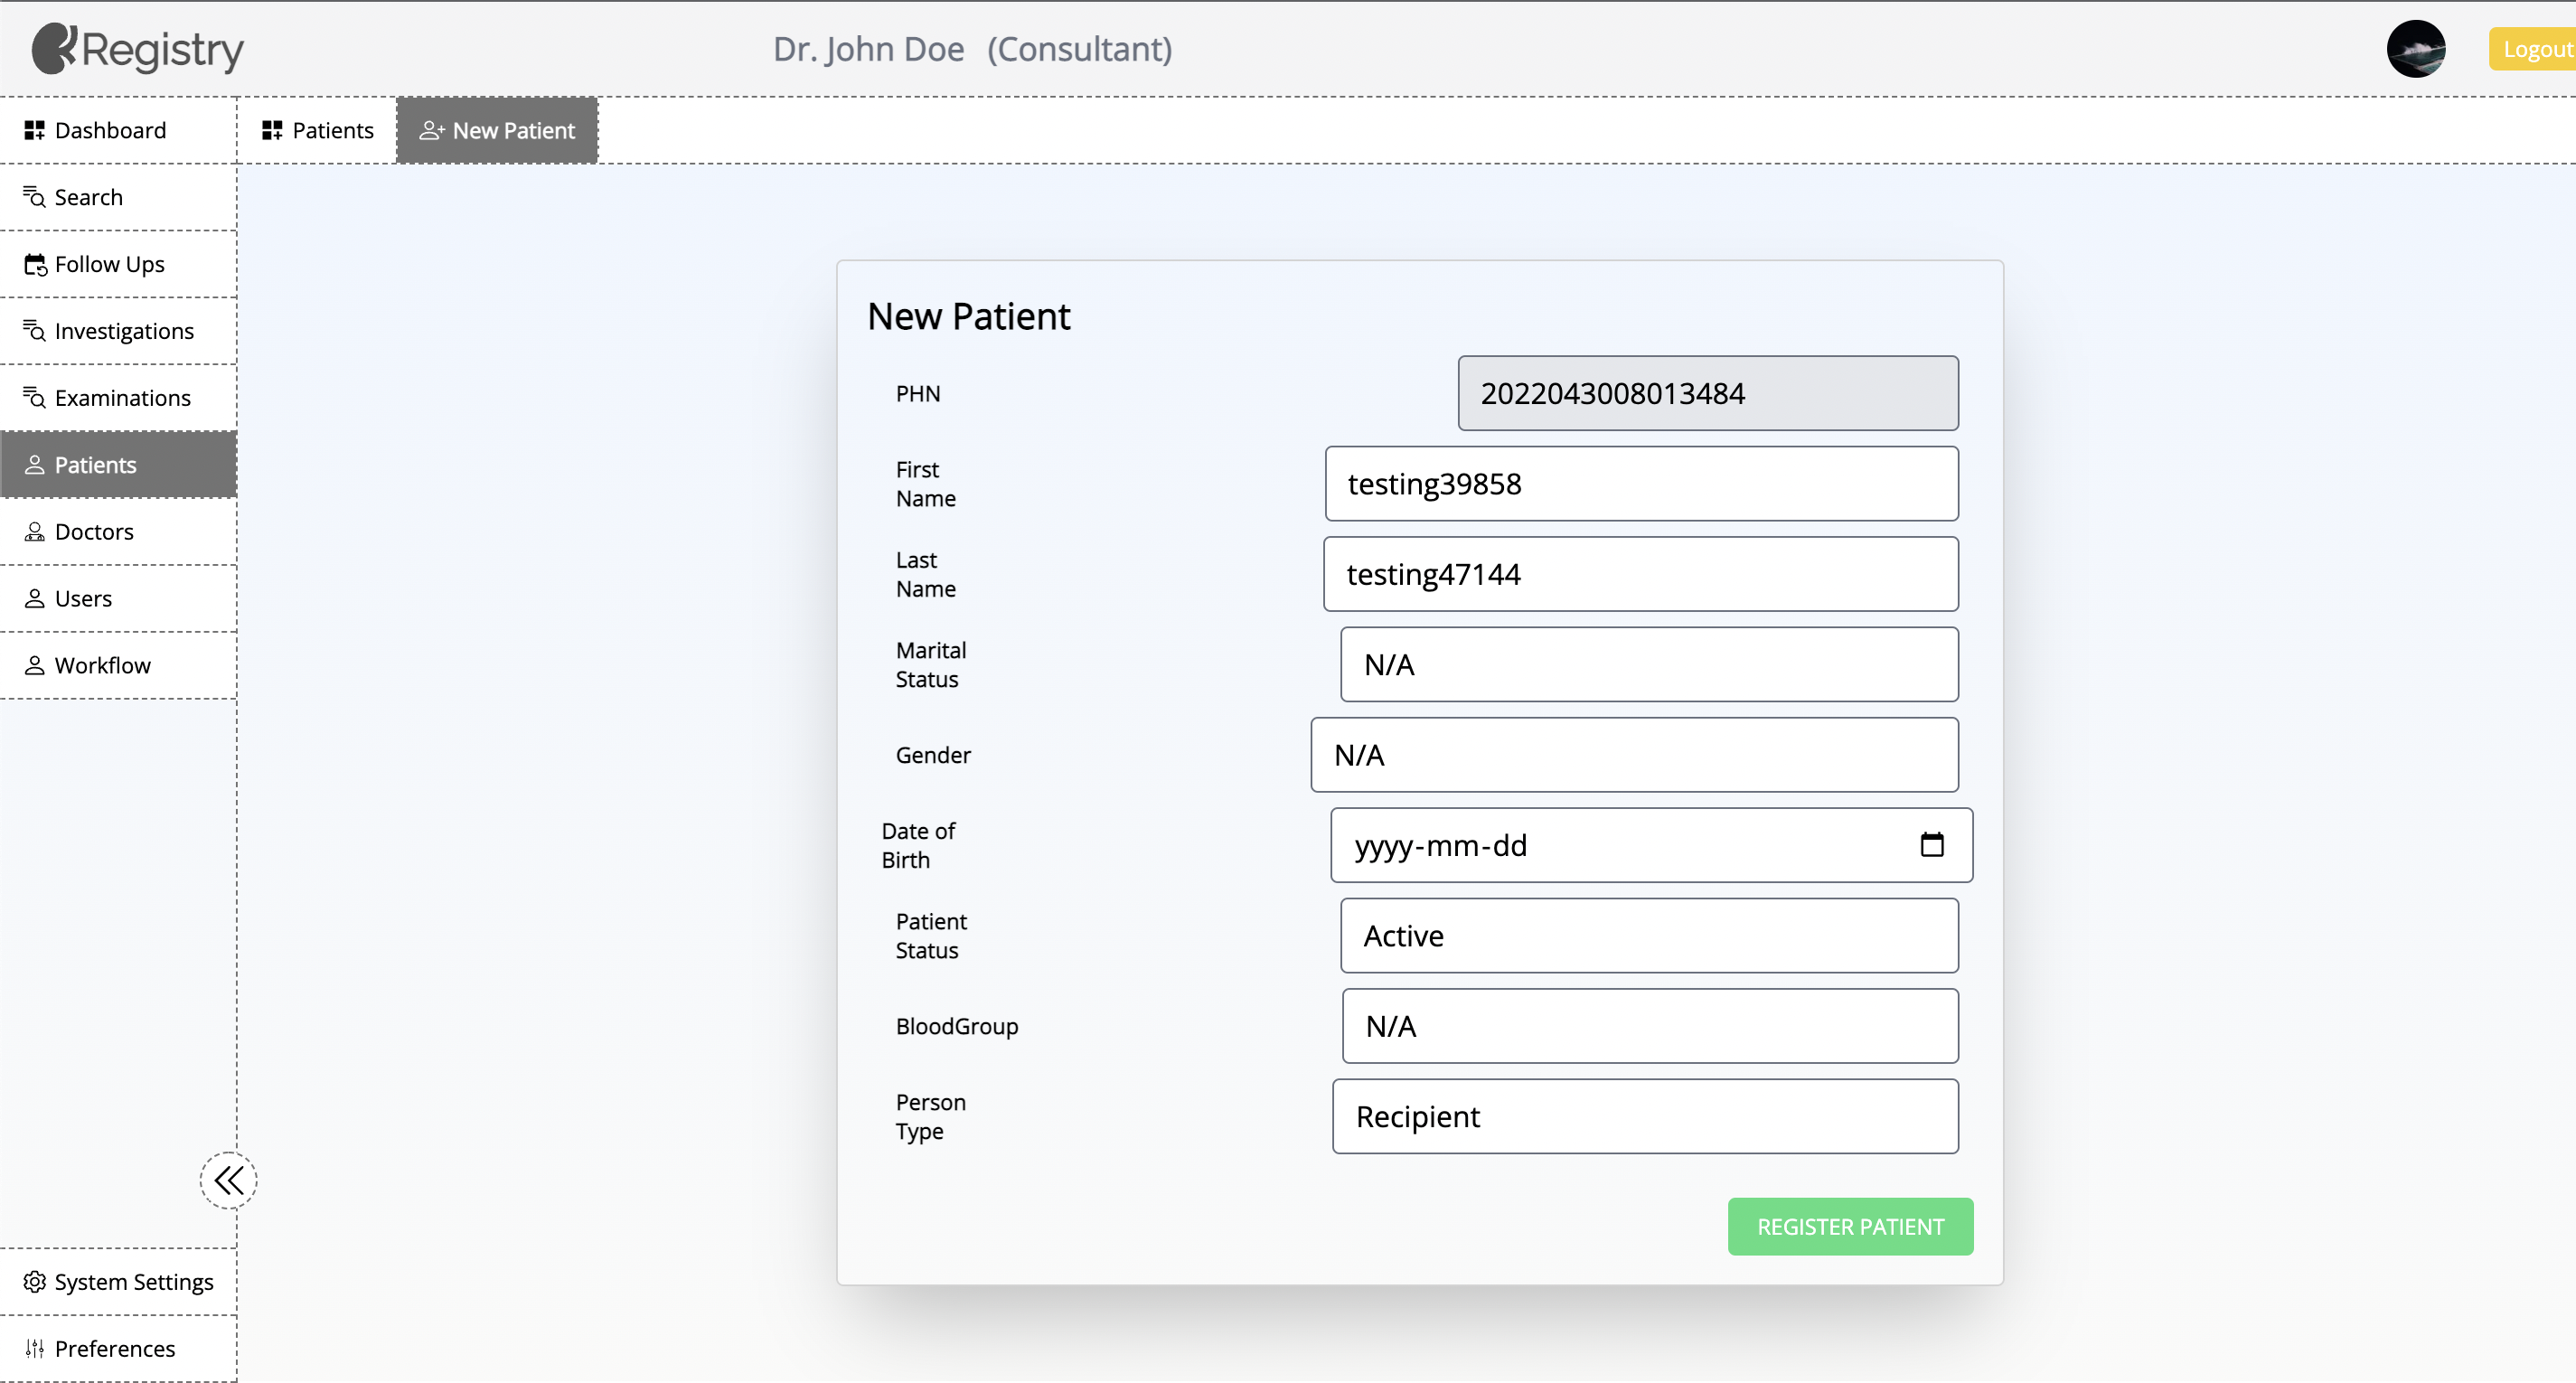
\includegraphics[width=0.8\textwidth]{images/patient-reg-layout.png}	
%\end{center}
%\caption{Patient Registration Screen}
%\label{fig:patient-registration-screen}
%\end{figure}

%\chapter*{Glossary}
%\addcontentsline{toc}{chapter}{Glossary}
%\printglossary[type=\acronymtype]

\printbibliography[nottype=book,heading=bibliography,title={References}]


\end{document}

